%Suitability of Exciters for Perceptual Control
%	Parameterise feature changes in terms of harmonic excitation.
%	Most suitable methods for given feature manipulations.
%	Easiest features to control in isolation.

\chapter{Controlling Audio Features} % control of low level features using exciters
\label{chap:FeatureControl}

\section{Introduction}
\label{sec:FeatureControl-Introduction}
	As discussed in Section \ref{sec:Timbre-Control}, previous studies have attempted to control perceptual features by
	controlling specific audio features. This chapter will identify the audio features which can be controlled through
	harmonic excitation and which excitation algorithms are the most suitable for given feature changes. 

\section{Harmonic Excitation Systems}
\label{sec:FeatureControl-Systems}
	Section \ref{sec:Excitation-Methods} covered several different methods of introducing new frequency content to a
	signal. Systems which combine these techniques with filtering afford a lot of control over the shape of a signal's
	spectrum. This section discusses the construction of these harmonic excitation systems. These systems discussed aim
	to give the user more control over the new content added to the spectrum producing a system which can be applied to
	as many use cases as possible.

	\subsection{Fundamental Frequency Tracking}
	\label{sec:FeatureControl-Systems-Fundamental}
		The majority of the methods discussed in Section \ref{sec:Excitation-Methods} will cause intermodulation
		distortion when used on signals with multiple frequency components. As the effects of this intermodulation
		distortion can be difficult to predict it can be useful to eliminate it altogether. This should make the
		effects of a system more predictable allowing it to be used in more situations.

		An simple way to achieve this is to process only the fundamental frequency of a signal. The fundamental of
		a signal can be isolated with a filter to produce a sinusoidal signal. A harmonic excitation method is then
		used to introduce harmonics to the fundamental. As the input is sinusoidal no intermodulation components
		will be produced. This `excited' signal is then summed with the original signal to produce the output. A
		diagram of this system is shown in Figure \ref{fig:F0Tracking}.

		\begin{figure}[h!]
			\centering
			\begin{tikzpicture}
				\node (In) at (0, 1) {$x[n]$};
				\coordinate (InMid) at (1, 1);
				\draw (In) -- (InMid);

				\coordinate (Through) at (1, 0);
				\draw (InMid) -- (Through);
				\coordinate (ThroughOut) at (9.5, 0);
				\draw (Through) -- (ThroughOut);

				\coordinate (Side) at (1, 2);
				\draw (InMid) -- (Side);

				\node (F0) [draw] at (3, 2) {Fundamental Tracker};
				\node (Filter) [draw] at (3, 1) {LPF};
				\draw (InMid) -- (Filter);
				\draw (F0) -- (Filter);

				\node (Exciter) [draw] at (5.5, 1) {Harmonic Exciter};
				\draw (Filter) -- (Exciter);
				\draw (Side) -- (F0);

				\node (Add) [operator] at (9.5, 1) {+};
				\draw (ThroughOut) -- (Add);

				\node (Gain) [gain] at (8, 1) {Gain};
				\draw (Exciter) -- (Gain);
				\draw (Gain) -- (Add);

				\node (Out) at (10.5, 1) {$y[n]$};
				\draw (Add) -- (Out);
			\end{tikzpicture}
			\caption{Fundamental frequency tracking in a harmonic excitation system.}
			\label{fig:F0Tracking}
		\end{figure}

		In order to use this method the fundamental frequency of a signal must be known in order to create a filter
		to isolate it. Fundamental tracking is a widely researched field and several algorithms have been presented
		in the literature several of which are reviewed by \citet{cuadra2001efficient} and
		\citet{gerhard2003pitch}.

		Fundamental tracking can be done in both the time and frequency domains. The simplest method being to count
		the number of instances of a particular event in a given time period. This even could be a zero crossing or
		a peak or any other easily identifiable feature of the signal. As signals get more complex this method
		becomes more difficult to apply as higher frequency content will produce more instances of the event being
		counted. More advanced time domain methods include the Average Magnitude Difference Function (AMDF) and
		autocorrelation methods. Many modern fundamental tracking systems are based on these, such as the VT-AMDF
		algorithm proposed by \citet{prukkanon2009vt-amdf}.

		These methods require frame based processing which reduces the time resolution of the system. If analysing
		real time audio the current estimate of the fundamental frequency will lag behind the audio signal.
		\citet{larsen2004audio} describe a time domain frequency tracker which uses a simple recursive formula.
		While this is not a accurate as the more advanced techniques it takes considerably less time to compute.

		Frequency domain methods require the DFT of the signal to be calculated introducing considerable
		complexity. Widely used frequency domain techniques include the Harmonic Product Spectrum (HPS) and maximum
		likelihood methods.

		For real time harmonic excitation the accuracy of the fundamental tracking algorithm is not as important as
		it is in other fields such as automatic music transcription. The aim of the system in Figure
		\ref{fig:F0Tracking} is to reduce the level of higher harmonics compared to the fundamental. Using a low
		pass filter with a cutoff frequency close to the fundamental will achieve this. The lag between the audio
		and the estimate of the fundamental frequency is of more concern. The system needs to respond quickly to
		changes in fundamental frequency in order to better isolate the fundamental for processing.

		A problem is posed by signals with little energy at their fundamental frequency such as those produce in
		the lower register of a Double Bass \citep{askenfelt2010double}. A fundamental tracking algorithm will
		still return the frequency of the fundamental despite its low magnitude. The output of the filter may then
		have to little amplitude to be of any use for harmonic excitation. A frequency domain approach to
		fundamental tracking may be more robust in this situation as it can easily be check whether there is
		sufficient energy at the detected fundamental frequency. If there is not, the first harmonic which has
		sufficient magnitude can be isolated and used as the input to the exciter. If this action is taken only the
		spectral replication and spectral shifting methods will allow for the excitation of every harmonic as the
		SSBA and IAP methods only allow for integer multiplications of the frequency.

		The system shown in Figure \ref{fig:F0Tracking} can provide differing levels of flexibility depending on
		the harmonic exciter used. Using a simple clipper it will generate a series of harmonics of the
		fundamental. Using methods which provide more control over the order of distortion allows users to excite
		single harmonics in the output. This will be covered in the next section.

	\subsection{Individual Harmonic Generation}
	\label{sec:FeatureControl-Systems-Individuals}
		Control over which harmonics are excited in a signal can be achieved by exciting individual harmonics. The
		principle behind this is to isolate the fundamental and then shift its frequency to that of the desired
		harmonic. This can be achieved using the SSBA, IAP, Spectral Replication and Spectral Stretching methods.
		The output spectrum can be shaped as desired by generating several different harmonics in this manner and
		summing them together.
		
		\citet{bregman1994auditory} suggests that when presented with an auditory scene the human hearing system
		separates out sources by grouping like harmonics together. Whether harmonics are deemed to be similar
		depends on their frequency and amplitude envelope. When applying harmonic excitation it is necessary to
		ensure that the newly introduced harmonic content will be judged as similar to the existing content. If not
		the excited harmonics may be perceived as a new sound source rather than contributing towards changing the
		timbre of a sound. Any system which generates new harmonic content and then sums it back into the original
		signal is at risk of this occurring. When generating multiple harmonics individually and summing them all
		together this risk is increased.

	\subsection{Spectral Shaping}
	\label{sec:FeatureControl-Systems-SpectralShaping}
		While generating individual harmonics allows for full control over the output spectrum it is very
		inefficient when a large number of new harmonics need to be introduced. For this purpose static
		nonlinearities prove useful. The characteristic curve of the nonlinearity can be designed to produce a set
		of harmonics with the desired qualities. The parity of the characteristic curve can be used to control
		whether odd or even harmonics are generated. The `smoothness' of the curve can also be adjusted to control
		the roll off of the harmonics amplitudes. The shape of the generated spectrum can then be further shaped by
		filtering.

		A spectral shaping system can be constructed in which a static nonlinearity and filter are used to excite a
		certain set of harmonics and finer control is provided using the individual harmonic generation techniques
		discussed in Section \ref{sec:FeatureControl-Systems-Individuals}. This allows the majority of the
		harmonics to be excited in an efficient manner only using more complex processing where it is needed.

		\citet{howard2009acoustics} discusses how low order harmonics sit in separate critical bands whereas high
		order harmonics are within one critical bandwidth of one another. This means that lower order harmonics are
		resolved separately by the human hearing system while the high order harmonics are perceived as fused
		sounds. As the order of harmonics increases their individual amplitudes have less effect on the perceived
		timbre of the sound. For this reason a harmonic excitation system need only provide control over the
		individual amplitudes of low order harmonics. 

		Using Equation \ref{eq:ERB} the minimum order for which harmonics lie within one critical bandwidth of one
		another can be calculated. For a signal with a given fundamental frequency, $f_{0}$, this order, $n$, can
		be calculated using the inequality in Equation \ref{eq:MinimumFusedHarmonic}.

		\[ f_{0} < 24.7 \left( 4.37n \frac{f_{0}}{1000} + 1 \right) \]
		\begin{equation}
			n > 1000 \frac{f_{0} - 24.7}{24.7 \times 4.37f_{0}}
			\label{eq:MinimumFusedHarmonic}
		\end{equation}

		This value is dependant on the fundamental frequency of the signal. As the frequency rises the minimum
		value of $n$ asymptotically grows towards 9.26 as shown in Equation \ref{eq:IndividualHarmonicLimit}.

		\begin{equation}
			\lim_{f_{0} \to \infty} 1000 \frac{f_{0} - 24.7}{24.7 \times 4.37f_{0}} \approx 9.26
			\label{eq:IndividualHarmonicLimit}
		\end{equation}

		This leads to the system shown in Figure \ref{fig:SpectralShapingSystem}. This is an expansion of the
		system shown in Figure \ref{fig:F0Tracking} providing finer control over the amplitudes of the low order
		harmonics.  The fundamental frequency is isolated in the same manner but several exciters are used in
		parallel.

		\begin{figure}[h!]
			\centering
			\begin{tikzpicture}
				\node (In) at (-1, -1.75) {$x[n]$};
				\coordinate (InMid) at (0, -1.75);
				\draw (In) -- (InMid);

				\coordinate (Side) at (0, -0.75);
				\draw (InMid) -- (Side);

				\node (F0) [draw] at (2, -0.75) {Fundamental Tracker};
				\node (F0Filter) [draw] at (2, -1.75) {LPF};
				\draw (InMid) -- (F0Filter);
				\draw (F0) -- (F0Filter);
				\draw (Side) -- (F0);

				\node (Add) [operator] at (10.5, -1.75) {+};

				\coordinate (ExciterIn) at (4, -1.75);
				\draw (F0Filter) -- (ExciterIn);

				% the fundamental
				\coordinate (F0In) at (4, 1);
				\node (F0Gain) [gain] at (9, 1) {};
				\draw (F0In) -- (F0Gain);
				\coordinate (F0Out) at (9.5, 1);
				\draw (F0Gain) -- (F0Out);
				\draw (F0Out) -- (Add);

				% second harmonic
				\coordinate (F1In) at (4, 0);
				\draw (F0In) -- (F1In);
				\node (F1) [draw] at (6.5, 0) {2\super{nd} Harmonic};
				\draw (F1In) -- (F1);

				\node (F1Gain) [gain] at (9, 0) {};
				\draw (F1) -- (F1Gain);
				\coordinate (F1Out) at (9.5, 0);
				\draw (F1Gain) -- (F1Out);
				\draw (F1Out) -- (Add);

				% third harmonic
				\coordinate (F2In) at (4, -1);
				\draw (F1In) -- (F2In);
				\node (F2) [draw] at (6.5, -1) {3\super{rd} Harmonic};
				\draw (F2In) -- (F2);

				\node (F2Gain) [gain] at (9, -1) {};
				\draw (F2) -- (F2Gain);
				\coordinate (F2Out) at (9.5, -1);
				\draw (F2Gain) -- (F2Out);
				\draw (F2Out) -- (Add);

				% ninth harmonic
				\coordinate (F8In) at (4, -2.5);
				\draw (F2In) -- (F8In);
				\node (F8) [draw] at (6.5, -2.5) {9\super{th} Harmonic};
				\draw (F8In) -- (F8);

				\node (F8Gain) [gain] at (9, -2.5) {};
				\draw (F8) -- (F8Gain);
				\coordinate (F8Out) at (9.5, -2.5);
				\draw (F8Gain) -- (F8Out);
				\draw (F8Out) -- (Add);

				\draw [dots] (F2) -- (F8);
				\draw [dots] (F2Gain) -- (F8Gain);

				% high order harmonics
				\coordinate (HighIn) at (4, -3.5);
				\draw (F8In) -- (HighIn);
				\node (High) [draw] at (5.7, -3.5) {Nonlinear Device};
				\draw (HighIn) -- (High);

				\node (HighFilter) [draw] at (8, -3.5) {Filter};
				\draw (High) -- (HighFilter);

				\node (HighGain) [gain] at (9, -3.5) {};
				\draw (HighFilter) -- (HighGain);
				\coordinate (HighOut) at (9.5, -3.5);
				\draw (HighGain) -- (HighOut);
				\draw (HighOut) -- (Add);

				% through
				\coordinate (Through) at (0, -4.5);
				\draw (InMid) -- (Through);
				\node (ThroughGain) [gain] at (9, -4.5) {};
				\draw (Through) -- (ThroughGain);
				\coordinate (ThroughOut) at (9.5, -4.5);
				\draw (ThroughGain) -- (ThroughOut);
				\draw (ThroughOut) -- (Add);

				\node (Out) at (11.5, -1.75) {$y[n]$};
				\draw (Add) -- (Out);
			\end{tikzpicture}
			\caption{An excitation system for controlling spectral structure.}
			\label{fig:SpectralShapingSystem}
		\end{figure}

		Each of the first nine harmonics are generated individually from the isolated fundamental. Higher order
		harmonics are generated using a static nonlinearity and filter in combination. The filter's primary purpose
		is to remove any energy present in the first nine harmonics but can also be used to alter the distribution
		of energy in the higher order harmonics.

	\subsection{Superposition}
	\label{sec:FeatureControl-Systems-Superposition}
		When processing musical systems additional challenges are met when attempting to shape the spectrum through
		excitation. One such challenge concerns the superposition of the existing harmonics in a signal and those
		produced by the excitation. In certain situations these two signals may cause destructive interference.
		Although the exciter is set to produce energy at a given harmonic when the signals are summed the energy at
		this harmonic decreases. To calculate the final amplitude of a harmonic after the excited signals have been
		summed with the original signal the phases and amplitudes of that harmonic in the original and excited
		signals must be known. This involves performing a full spectral analysis on the input signal. 

		When using a system like that shown in Figure \ref{fig:SpectralShapingSystem} the phases and amplitudes of
		the excited harmonics depend on the phase and amplitude of the fundamental frequency after the low pass
		filter. Using the SSBA and IAP techniques, to generate the $n$\super{th} harmonic, the phase of the output
		is $n$ times that of the input after the Hilbert transform filter has been applied. The phases of the
		harmonics produced by a static nonlinearity can be determined by calculating the Fourier series of a
		sinusoid with the nonlinearity applied.

		Calculating this in real time dramatically increases the computational complexity of the system. This
		complexity can be avoided by avoiding superposition of harmonics. This simplest way to achieve this is by
		discarding the original signal and constructing the output from only the fundamental and generated
		harmonics. This destroys most of the timbral characteristics of a signal, completely reconstructing its
		spectrum. For situations where a dramatic alteration of timbre is desired this can be a useful technique
		but for more subtle timbral manipulations it is better to preserve more of the original spectral structure.

		A less intrusive method is to filter energy out of the input signal only at the frequencies which are to be
		excited. For the system in Figure \ref{fig:SpectralShapingSystem} this can be implemented using a series of
		notch filters tuned to the frequencies of the first nine harmonics and a low pass filter to attenuate any
		frequency above the ninth harmonic. These filters can be applied to the unexcited signal depending on which
		harmonics are being generated by the exciters. A diagram of a system which includes these filters is shown
		in Figure \ref{fig:SuperpositionSystem}.

		\begin{figure}[h!]
			\centering
			\begin{tikzpicture}
				\node (In) at (-1, -1.75) {$x[n]$};
				\coordinate (InMid) at (0, -1.75);
				\draw (In) -- (InMid);

				\coordinate (Side) at (0, -0.75);
				\draw (InMid) -- (Side);

				\node (F0) [draw] at (2, -0.75) {Fundamental Tracker};
				\node (F0Filter) [draw] at (2, -1.75) {LPF};
				\draw (InMid) -- (F0Filter);
				\draw (F0) -- (F0Filter);
				\draw (Side) -- (F0);

				\node (Add) [operator] at (10.5, -1.75) {+};

				\coordinate (ExciterIn) at (4, -1.75);
				\draw (F0Filter) -- (ExciterIn);

				% the fundamental
				\coordinate (F0In) at (4, 1);
				\node (F0Gain) [gain] at (9, 1) {};
				\draw (F0In) -- (F0Gain);
				\coordinate (F0Out) at (9.5, 1);
				\draw (F0Gain) -- (F0Out);
				\draw (F0Out) -- (Add);

				% second harmonic
				\coordinate (F1In) at (4, 0);
				\draw (F0In) -- (F1In);
				\node (F1) [draw] at (6.5, 0) {2\super{nd} Harmonic};
				\draw (F1In) -- (F1);

				\node (F1Gain) [gain] at (9, 0) {};
				\draw (F1) -- (F1Gain);
				\coordinate (F1Out) at (9.5, 0);
				\draw (F1Gain) -- (F1Out);
				\draw (F1Out) -- (Add);

				% third harmonic
				\coordinate (F2In) at (4, -1);
				\draw (F1In) -- (F2In);
				\node (F2) [draw] at (6.5, -1) {3\super{rd} Harmonic};
				\draw (F2In) -- (F2);

				\node (F2Gain) [gain] at (9, -1) {};
				\draw (F2) -- (F2Gain);
				\coordinate (F2Out) at (9.5, -1);
				\draw (F2Gain) -- (F2Out);
				\draw (F2Out) -- (Add);

				% ninth harmonic
				\coordinate (F8In) at (4, -2.5);
				\draw (F2In) -- (F8In);
				\node (F8) [draw] at (6.5, -2.5) {9\super{th} Harmonic};
				\draw (F8In) -- (F8);

				\node (F8Gain) [gain] at (9, -2.5) {};
				\draw (F8) -- (F8Gain);
				\coordinate (F8Out) at (9.5, -2.5);
				\draw (F8Gain) -- (F8Out);
				\draw (F8Out) -- (Add);

				\draw [dots] (F2) -- (F8);
				\draw [dots] (F2Gain) -- (F8Gain);

				% high order harmonics
				\coordinate (HighIn) at (4, -3.5);
				\draw (F8In) -- (HighIn);
				\node (High) [draw] at (5.7, -3.5) {Nonlinear Device};
				\draw (HighIn) -- (High);

				\node (HighFilter) [draw] at (8, -3.5) {Filter};
				\draw (High) -- (HighFilter);

				\node (HighGain) [gain] at (9, -3.5) {};
				\draw (HighFilter) -- (HighGain);
				\coordinate (HighOut) at (9.5, -3.5);
				\draw (HighGain) -- (HighOut);
				\draw (HighOut) -- (Add);

				% through
				\coordinate (Through) at (0, -4.5);
				\draw (InMid) -- (Through);
				\node (ThroughFilter) [draw] at (8, -4.5) {Filter};
				\draw (Through) -- (ThroughFilter);
				\node (ThroughGain) [gain] at (9, -4.5) {};
				\draw (ThroughFilter) -- (ThroughGain);
				\coordinate (ThroughOut) at (9.5, -4.5);
				\draw (ThroughGain) -- (ThroughOut);
				\draw (ThroughOut) -- (Add);

				\node (Out) at (11.5, -1.75) {$y[n]$};
				\draw (Add) -- (Out);
			\end{tikzpicture}
			\caption{The system from Figure \ref{fig:SpectralShapingSystem} extended to allow for filtering of
				 the original signal.}
			\label{fig:SuperpositionSystem}
		\end{figure}

		Removing harmonics from the original signal looses any phase information that was present for those
		frequencies. The newly generated harmonics may not have the same phase as those that have been removed
		potentially causing unwanted timbral effects. The phases of a signal's partials influence its temporal
		features. \citet{plomp1969effect} discuss the audible effects of this for harmonic signals, concluding that
		the effect is more subtle than, but independent to, that of changing the harmonics' amplitudes. They state
		that the largest perceptual difference occurs between a signal in which all the harmonics have the same
		phase and one composed of harmonics with phases alternating between two values $\frac{\pi}{2}$ radians
		apart.

		For fine control it may be beneficial to separate control of the amplitude and phase of each partial in a
		signal. This is most easily achieved using the IAP technique as the phase of the input signal is already
		exposed in the calculation. Introducing a phase parameter, $\theta$, to Equation \ref{eq:IAP} gives rise to
		Equation \ref{eq:IAPWithPhase}.

		\begin{equation}
			y[n] = \abs{x_{a}[n]} \cos \left( h\arg(x_{a}[n] + \theta) \right), \quad h \in \textbf{N}
			\label{eq:IAPWithPhase}
		\end{equation}

		Assuming a sinusoidal input this new parameter controls the phase of the generated harmonic relative to
		that of the input. 
		
		For introducing new spectral content with a specific amplitude and phase Equation \ref{eq:IAPWithPhase}
		suffices. Separate control of the phase and amplitudes of existing partials can be achieved in two ways.
		The first is to use an analysis / resynthesis system in which the amplitudes and phases of the partials are
		adjusted in the frequency domain. The second approach is to use zero phase filters to amplify or attenuate
		partials and phase shifting techniques to adjust their phases. Both of these approaches introduce delay
		into the system be it through the windowing used for spectral analysis or the delay introduced to make
		filters causal.

		\note
		{
			Perhaps add these filters and things to the system diagram.
		}

	\subsection{Inharmonicity}
	\label{sec:FeatureControl-Systems-Inharmonicity}
		With a sinusoidal input the SSBA and IAP techniques generate perfectly harmonic partials. As inharmonicity
		is an important cue for differentiating timbre it is desirable to be able to introduce some inharmonicity
		to the generated partials.

		Spectral replication allows for generation of partials at any frequency, but in order for their frequency
		to be accurate the exact fundamental frequency must be known. This causes the system to rely on the
		accuracy of the fundamental frequency tracking algorithm used meaning a much more complex tracker needs to
		be used adding to the complexity of the system. A system which provides control over inharmonicity and does
		not rely on accurate fundamental tracking is shown in Figure \ref{fig:InharmonicitySystem}.

		\begin{figure}[h!]
			\centering
			\begin{tikzpicture}
				\node (In) at (-1, -1.75) {$x[n]$};
				\coordinate (InMid) at (0, -1.75);
				\draw (In) -- (InMid);

				\coordinate (Side) at (0, -0.75);
				\draw (InMid) -- (Side);

				\node (F0) [draw] at (2, -0.75) {Fundamental Tracker};
				\node (F0Filter) [draw] at (2, -1.75) {LPF};
				\draw (InMid) -- (F0Filter);
				\draw (F0) -- (F0Filter);
				\draw (Side) -- (F0);

				\node (Add) [operator] at (11.5, -1.75) {+};

				\coordinate (ExciterIn) at (4, -1.75);
				\draw (F0Filter) -- (ExciterIn);

				\node (LPF) [draw] at (2, -3.5) {LPF};

				% the fundamental
				\coordinate (F0In) at (4, 1);
				\node (F0Gain) [gain] at (10, 1) {};
				\draw (F0In) -- (F0Gain);
				\coordinate (F0Out) at (10.5, 1);
				\draw (F0Gain) -- (F0Out);
				\draw (F0Out) -- (Add);

				% second harmonic
				\coordinate (F1In) at (4, 0);
				\draw (F0In) -- (F1In);
				\node (F1) [draw] at (6, 0) {2\super{nd} Harmonic};
				\draw (F1In) -- (F1);

				\node (F1Shifter) [draw] at (8.5, 0) {Shifter};
				\draw (F1) -- (F1Shifter);

				\node (F1Gain) [gain] at (10, 0) {};
				\draw (F1Shifter) -- (F1Gain);
				\coordinate (F1Out) at (10.5, 0);
				\draw (F1Gain) -- (F1Out);
				\draw (F1Out) -- (Add);

				% third harmonic
				\coordinate (F2In) at (4, -1);
				\draw (F1In) -- (F2In);
				\node (F2) [draw] at (6, -1) {3\super{rd} Harmonic};
				\draw (F2In) -- (F2);

				\node (F2Shifter) [draw] at (8.5, -1) {Shifter};
				\draw (F2) -- (F2Shifter);

				\node (F2Gain) [gain] at (10, -1) {};
				\draw (F2Shifter) -- (F2Gain);
				\coordinate (F2Out) at (10.5, -1);
				\draw (F2Gain) -- (F2Out);
				\draw (F2Out) -- (Add);

				% ninth harmonic
				\coordinate (F8In) at (4, -2.5);
				\draw (F2In) -- (F8In);
				\node (F8) [draw] at (6, -2.5) {9\super{th} Harmonic};
				\draw (F8In) -- (F8);

				\node (F8Shifter) [draw] at (8.5, -2.5) {Shifter};
				\draw (F8) -- (F8Shifter);

				\node (F8Gain) [gain] at (10, -2.5) {};
				\draw (F8Shifter) -- (F8Gain);
				\coordinate (F8Out) at (10.5, -2.5);
				\draw (F8Gain) -- (F8Out);
				\draw (F8Out) -- (Add);

				\draw [dots] (F2) -- (F8);
				\draw [dots] (F2Shifter) -- (F8Shifter);
				\draw [dots] (F2Gain) -- (F8Gain);

				% high order harmonics
				\coordinate (HighIn) at (0, -3.5);
				\node (High) [draw] at (6, -3.5) {Nonlinear Device};
				\draw (LPF) -- (High);
				\draw (HighIn) -- (LPF);

				\node (HighFilter) [draw] at (8.5, -3.5) {Filter};
				\draw (High) -- (HighFilter);

				\node (HighGain) [gain] at (10, -3.5) {};
				\draw (HighFilter) -- (HighGain);
				\coordinate (HighOut) at (10.5, -3.5);
				\draw (HighGain) -- (HighOut);
				\draw (HighOut) -- (Add);

				% through
				\coordinate (Through) at (0, -4.5);
				\draw (InMid) -- (Through);
				\node (ThroughFilter) [draw] at (8.5, -4.5) {Filter};
				\draw (Through) -- (ThroughFilter);
				\node (ThroughGain) [gain] at (10, -4.5) {};
				\draw (ThroughFilter) -- (ThroughGain);
				\coordinate (ThroughOut) at (10.5, -4.5);
				\draw (ThroughGain) -- (ThroughOut);
				\draw (ThroughOut) -- (Add);

				\node (Out) at (12.5, -1.75) {$y[n]$};
				\draw (Add) -- (Out);
			\end{tikzpicture}
			\caption{An extension of the system in Figure \ref{fig:SuperpositionSystem} to allow for control
			         of inharmonicity.}
			\label{fig:InharmonicitySystem}
		\end{figure}

		As in Figure \ref{fig:SpectralShapingSystem} the second through ninth harmonics are generated individually.
		This can be done using any method which generates accurate harmonics. Each harmonic is then shifted to the
		desired frequency using the single sideband modulation technique shown in Section
		\ref{sec:Excitation-Methods-SpectralReplication}. This produces partials which deviate from
		harmonic frequencies by exactly the amount of shift applied.

		The higher order harmonics are not generated individually and as such their inharmonicity cannot be
		controlled individually. Spectral replication could be used to shift their frequencies as is done with the
		lower order harmonics. This restricts the higher harmonics to all having the same degree of inharmonicity.
		This may sound unnatural as in natural tones the inharmonicity of a harmonic is typically dependant on the
		order of the harmonic (such as in piano tones \citep{young1952inharmonicity}).

		The system in Figure \ref{fig:InharmonicitySystem} provides an alternative method of introducing
		inharmonicity in the high order harmonics. A separate low pass filter is used to produce an input for the
		static nonlinearity. If this filter's cutoff frequency is set to isolate the fundamental frequency the
		nonlinearity will only produce harmonic distortion components. As the cutoff frequency in increased,
		allowing more partials of the input signal to pass through, the level of intermodulation distortion
		produced by the nonlinearity increases. The inharmonicity of these intermodulation components will depend
		on the inharmonicity of the partials in the input signal. This method of introducing inharmonicity is less
		controllable than using spectral replication but it will produce a different set of inharmonic partials
		about each harmonic frequency in the output signal. A considerable disadvantage is that it will only create
		inharmonicities for inputs which already contain a degree of inharmonicity.

\section{Parameterisation of Feature Changes}
\label{sec:FeatureControl-Parameterisation}
	The systems discussed in Section \ref{sec:FeatureControl-Systems} provide control over where energy is introduced
	in a signal's spectrum. Large bands of energy can be introduced or finer control over specific harmonics can be
	provided. This section discusses how the control of low level audio features can be parameterised using these kinds
	of manipulations. The measurement of each audio feature is discussed and methods by which a single parameter can be
	used to adjust them are suggested.

	Assuming perfect detection of fundamental frequency and perfect filters, the systems shown in Section
	\ref{sec:FeatureControl-Systems}, along with the methods discussed in this Section, would provide accurate control
	over the audio features. In a `real world' implementation the properties of the input signal and filters used will
	affect how the features of manipulated. To examine these effects each method for manipulating a feature is tested
	on four harmonic audio signals produced by the following instruments:

	\begin{itemize}
		\item A bowed cello. \note{All harmonics}
		\item A clarinet. \note{Only Odd Harmonics}
		\item A synthesised harmonic sound. \note{Zero Inharmonicity}
		\item A piano. \note{Damped Fundamental}
	\end{itemize}

	\note{Why these samples?}

	Several of the audio features discussed involve analysis of a signals spectrum. To simplify the notation of these
	features it is useful to introduce the concept of a spectral component. A spectral component describes a part of
	the signals spectrum, be it a spectral bin obtained from a DFT, a partial of the signal, or a frequency band taken
	from the spectrum. In the following equations, unless otherwise stated, the symbols $a_{n}$ and $\nu_{n}$ will
	refer to the amplitude and frequency of the $n$\super{th} spectral component of a signal respectively. $N$ denotes
	the total number of spectral components in the signal.

	\subsection{Spectral Moments}
	\label{sec:FeatureControl-Parameterisation-SpectralMoments}
		The spectral moments are the statistical moments of a signals spectrum. They describe how the energy is
		distributed in a spectrum. The first four spectral moments are the centroid, spread, skewness and kurtosis.
		
		The spectral centroid of a signal, $\mu$, is the first raw moment (mean) of the spectrum. It is calculated
		using Equation \ref{eq:SpectralCentroid}.

		\begin{equation}
			\mu = \frac{\sum_{n = 1}^{N} \nu_{n}a_{n}}
				   {\sum_{n = 1}^{N} a_{n}}
			\label{eq:SpectralCentroid}
		\end{equation}

		The spectral spread of a signal, $\sigma^{2}$, is the second central moment (variance) of the
		spectrum. It is calculated using Equation \ref{eq:SpectralSpread}.

		\begin{equation}
			\sigma^{2} = \frac{\sum_{n = 1}^{N} a_{n}(\nu_{n} - \mu)^{2}}
					  {\sum_{n = 1}^{N} a_{n}}
			\label{eq:SpectralSpread}
		\end{equation}

		Together, the spectral centroid and spread give a description of where the energy in a spectrum is centered
		and how far from this center the energy is spread.

		The spectral skewness of a signal, $\gamma$, is the third standardised moment of the spectrum. It is
		calculated using Equation \ref{eq:SpectralSkewness}.

		\begin{equation}
			\gamma = \frac{\sum_{n = 1}^{N} a_{n}(\nu_{n} - \mu)^{3}}
				      {\sigma^{3}\sum_{n = 1}^{N} a_{n}}
			\label{eq:SpectralSkewness}
		\end{equation}

		The spectral skewness measure how symmetrical a spectrum is about its centroid. A negative skewness
		describes a spectrum with more energy above its centroid while a positive skewness describes the opposite.
		A skewness of zeros describes a spectrum with equal energy either side of its centroid.

		The spectral kurtosis of a signal, $\kappa$, is the fourth standardised moment of the spectrum. It
		is calculated using Equation \ref{eq:SpectralKurtosis}.

		\begin{equation}
			\kappa = \frac{\sum_{n = 1}^{N} a_{n}(\nu_{n} - \mu)^{4}}
				      {\sigma^{4}\sum_{n = 1}^{N} a_{n}}
			\label{eq:SpectralKurtosis}
		\end{equation}

		The kurtosis measures the length of a distributions tails. A low kurtosis describes a spectrum where the
		energy in evenly distributed in a band around the centroid. A high kurtosis describes a spectrum in which
		small amounts of energy lies at frequencies far away from the central band.

		The kurtosis of a normal distribution is 3. This gives rise to a different measure, the excess kurtosis,
		which is defined as $\kappa - 3$. The excess kurtosis is often referred to as the kurtosis. This gives rise
		to some obscurity when reading literature which discusses the kurtosis without providing a definition.

		\subsubsection*{Manipulation of The Spectral Centroid}
			A crude method of causing the spectral centroid to move towards a particular frequency is the
			increase the energy at that frequency. While this works conceptually it is destructive to the
			original structure of the spectrum. As the centroid moves towards the desired frequency the
			spectrum is dominated by a sinusoid at that frequency.

			Less destructive methods include that used by \citet{zacharakis2011an} who split the signal into
			two bands, one above and one below the spectral centroid. The relative amplitudes of these bands
			can then be altered to adjust the spectral centroid. This preserves more of the original signals
			structure, the relative levels of partials within each band remaining the same. Using this method
			the new spectral centroid will lie somewhere between the respective centroids of the two bands. The
			relative amplitudes of the two bands required to give a certain spectral centroid, $\mu$, can be
			calculated using Equation \ref{eq:SpectralCentroidManipulation}.

			\begin{equation}
				\frac{\sum_{n = c + 1}^{N} a_{n}}
				     {{\sum_{n = 1}^{c} a_{n}}} = 
				\frac{\mu_{l} - \mu}{\mu - \mu_{u}}, 
				\quad \mu_{l} \leq \mu < \mu_{u} \quad \textrm{or} \quad \mu_{u} < \mu \leq \mu_{l}
				\label{eq:SpectralCentroidManipulation}
			\end{equation}

			Where $\mu_{l}$ and $\mu_{r}$ are the spectral centroid of the upper and lower band, and $c$ is the
			order highest frequency spectral component in the lower band.

			\citet{williams2007perceptually} employ a spectral tilt to manipulate spectral centroid, applying
			gain to the partials of a signal as a linear function of their frequency. This allows the spectral
			centroid to be moved up or down in frequency while still retaining the frequency content of the
			signal. A disadvantage of this method is that the change in centroid cannot be easily parameterised
			as it depends on the content of the signal being processed.

			Another way to move the spectral centroid is by introducing a new band of energy into the spectrum.
			This is conceptually similar to the two band method discussed previously but allows the second band
			to contain frequency content which was not in the original signal. As before the overall spectral
			centroid can be moved by adjusting the relative amplitudes of the original signal and the new band
			of energy. To facilitate accurate control of the spectral centroid these bands should not share any
			frequency components. Figure \ref{fig:TwoBandSpectralCentroidSystem} shows a system which
			separately controls the gains of two bands.

			\begin{figure}[h!]
				\centering
				\begin{tikzpicture}
					\node (In) at (0, 1) {$x[n]$};
					\coordinate (InMid) at (1, 1);
					\draw (In) -- (InMid);

					\coordinate (Through) at (1, 0);
					\draw (InMid) -- (Through);
					\node (ThroughFilter) [draw] at (5.5, 0) {LPF};
					\draw (Through) -- (ThroughFilter);
					\node (ThroughGain) [gain] at (9.25, 0) {};
					\draw (ThroughFilter) -- (ThroughGain);
					\coordinate (ThroughOut) at (10.5, 0);
					\draw (ThroughGain) -- (ThroughOut);

					\coordinate (Side) at (1, 2);
					\draw (InMid) -- (Side);

					\node (F0) [draw] at (3, 2) {Fundamental Tracker};
					\node (Filter) [draw] at (3, 1) {LPF};
					\draw (InMid) -- (Filter);
					\draw (F0) -- (Filter);

					\node (Exciter) [draw] at (5.5, 1) {Nonlinear Device};
					\draw (Filter) -- (Exciter);
					\draw (Side) -- (F0);

					\node (NldFilter) [draw] at (8, 1) {HPF};
					\draw (Exciter) -- (NldFilter);

					\node (Add) [operator] at (10.5, 1) {+};
					\draw (ThroughOut) -- (Add);

					\node (Gain) [gain] at (9.25, 1) {};
					\draw (NldFilter) -- (Gain);
					\draw (Gain) -- (Add);

					\node (Out) at (11.5, 1) {$y[n]$};
					\draw (Add) -- (Out);
				\end{tikzpicture}
				\caption{A system for controlling the spectral centroid.}
				\label{fig:TwoBandSpectralCentroidSystem}
			\end{figure}

			The lower band is generated via a low pass filter on the input signal while the high band is
			created using a nonlinear device. The bands are filtered with corresponding low and high pass
			filters to ensure they share no frequency components. The spectral centroid of the output can be
			moved between the centroids of these two bands by changing their relative gains according to
			Equation \ref{eq:SpectralCentroidManipulation}.

			This method has some advantages over manipulating the amplitudes of two bands using only linear
			filters. The centroid can be manipulated in various manners. The nonlinear device can be used to
			reconstruct the high frequency portion of the signal and the relative gains adjusted similarly to
			if two filters were used.  Alternatively the properties of the nonlinear device can be altered to
			change the upper band's centroid.  This provides more flexibility allowing the centroid to be
			changed independently of some other features. For example, changing the gains of two bands will
			change the spectral slope of the signal. If instead additional partials are introduced to the
			upper, with amplitudes which are determined by the signals current slope, the centroid can be move
			while the slope is unaltered.

			Figure \ref{fig:MoveCentroids} shows the effect of this system on the test signals. The parameter
			value corresponds to the gains applied to the two bands. Where the parameter value is $P$, the low
			band is multiplied by a gain of $1 - P$ and the high band by a gain of $P$.

			\begin{figure}[h!]
				\centering
				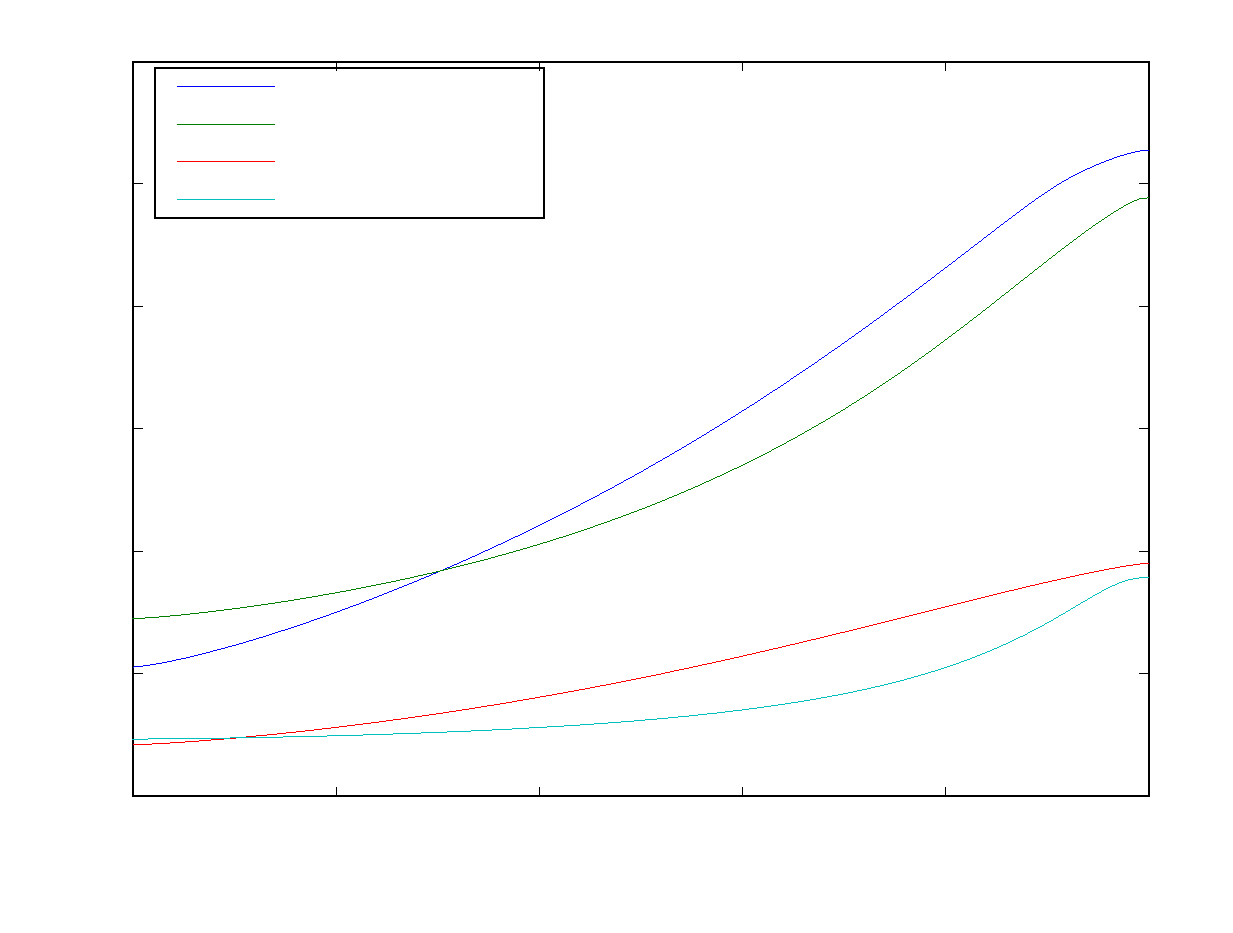
\includegraphics[width=0.6\textwidth]{chapter6/Images/MoveCentroids.eps}
				\caption{Manipulating the Spectral Centroids of the Test Signals.}
				\label{fig:MoveCentroids}
			\end{figure}

			\note{Probably discuss that graph.}

		\subsubsection*{Manipulation of The Higher Order Spectral Moments}
			Higher order spectral moments are more difficult to parameterise. The measures depend on the
			displacement of each spectral component from the centroid, skewness and kurtosis measurements also
			depend on the spectral spread. To simplify the control of these moments it is necessary to use
			manipulations which do not alter the moments they depend on. 
			
			Controlling the spread while keeping the centroid constant involves adding or removing energy
			symmetrically about the centroid. Deciding where to add or remove this energy is a complicated
			process. The frequencies of the spectral components are not likely to be symmetrical about the
			centroid meaning different gains must be applied to components either side of the centroid.
			Calculating these gains must be done on a signal by signal basis making if difficult to provide a
			general solution. These problems are compounded further when trying to control the higher order
			moments as the spectral spread must be kept constant as well.

			Intuition about what the spectral moments describe can be used to influence them in a simpler
			manner. These methods do not provide accurate control over a specific moment but allow it to be
			increased or decreased.  Furthermore, they will have an effect on all the spectral moments rather
			than one in isolation. 
			
			Spectral spread can be increased by adding energy at frequencies which are more that one spectral
			spread from the centroid or reducing the energy at frequencies within one spectral spread of the
			centroid.  Applying the opposite operations will decrease the spectral spread. This can be
			implemented using a system similar to that in Figure \ref{fig:TwoBandSpectralCentroidSystem}. A
			band of harmonic energy is generated by processing the isolated fundamental with a nonlinear device
			followed by a band pass filter. This new band can then be summed with the original signal at the
			desired gain. Figure \ref{fig:MoveSpreads} shows the change is spectral spread when the gain of a
			spectral band, containing energy between 0.8 and 1.2 of the spectral centroid, is changed.

			\begin{figure}[h!]
				\centering
				\includegraphics[width=0.6\textwidth]{chapter6/Images/MoveSpreads.eps}
				\caption{Manipulating the Spectral Spreads of the Test Signals.}
				\label{fig:MoveSpreads}
			\end{figure}

			\note{Describe that.}

			Spectral skewness can be increased by applying a spectral tilt. A tilt with a positive gradient
			will decrease the skewness, whereas a negative gradient will increase the skewness. While this is
			easily implemented using linear filters it can also be applied using the excitation system shown in
			Figure \ref{fig:InharmonicitySystem}. The levels of the individually generated harmonics can be
			adjusted in order to achieve the desired spectral tilt. Figure \ref{fig:MoveSkewnesses} shows the
			effect different gradients of spectral tilt on the spectral skewness of the test signals.

			\begin{figure}[h!]
				\centering
				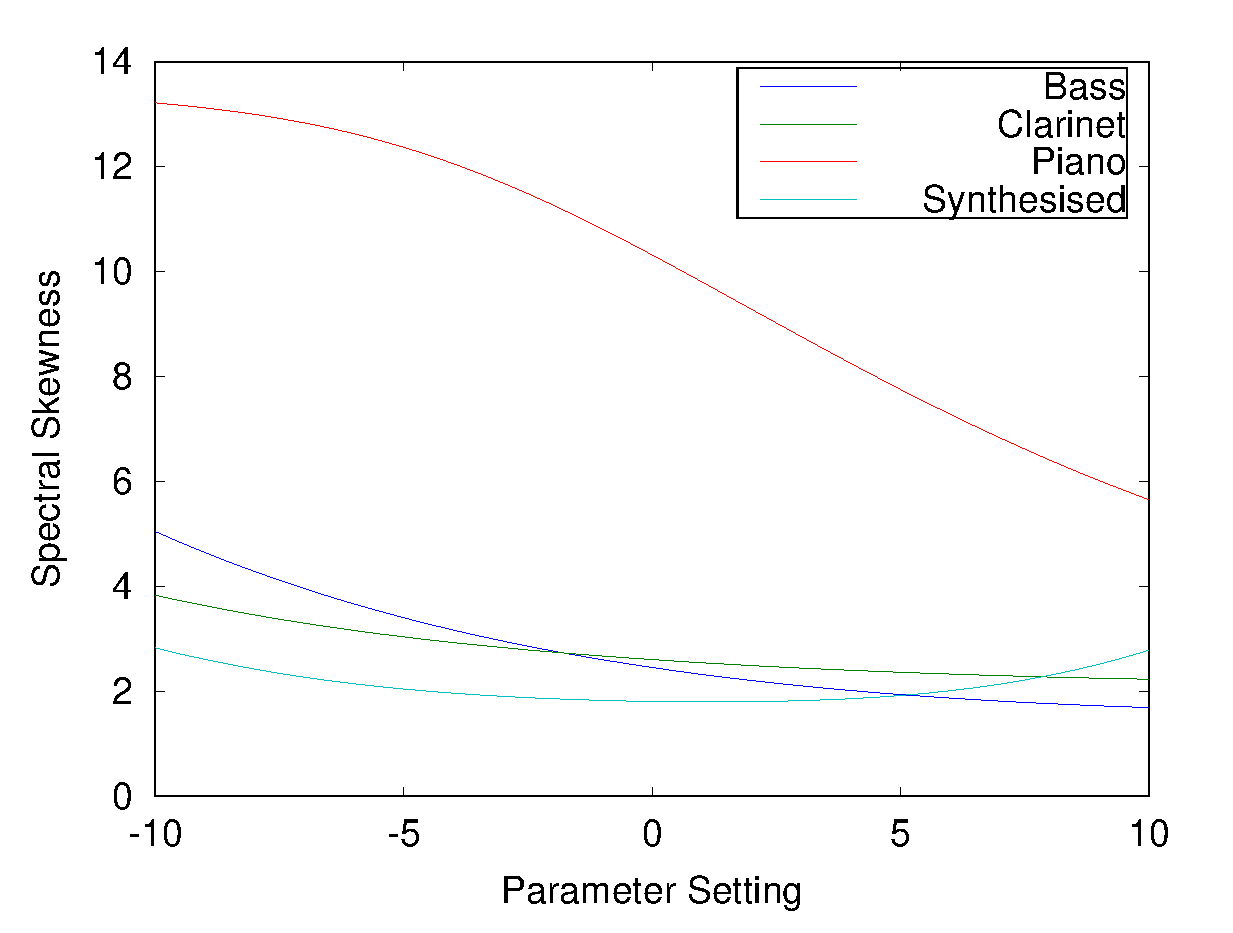
\includegraphics[width=0.6\textwidth]{chapter6/Images/MoveSkewnesses.eps}
				\caption{Manipulating the Spectral Skewnesses of the Test Signals.}
				\label{fig:MoveSkewnesses}
			\end{figure}

			\note{Some discussion. Why doesn't the skewness for the synthesiser change?}

			Spectral kurtosis can be changed using the same method as for spectral spread. Increasing the
			energy near the centroid reduces the kurtosis, while removing energy near the centroid increases
			the kurtosis. Figure \ref{fig:MoveKurtoses} shows the effect on the spectral kurtosis of the test
			signal when undergoing the same processing as described for Figure \ref{fig:MoveSpreads}.
			
			\begin{figure}[h!]
				\centering
				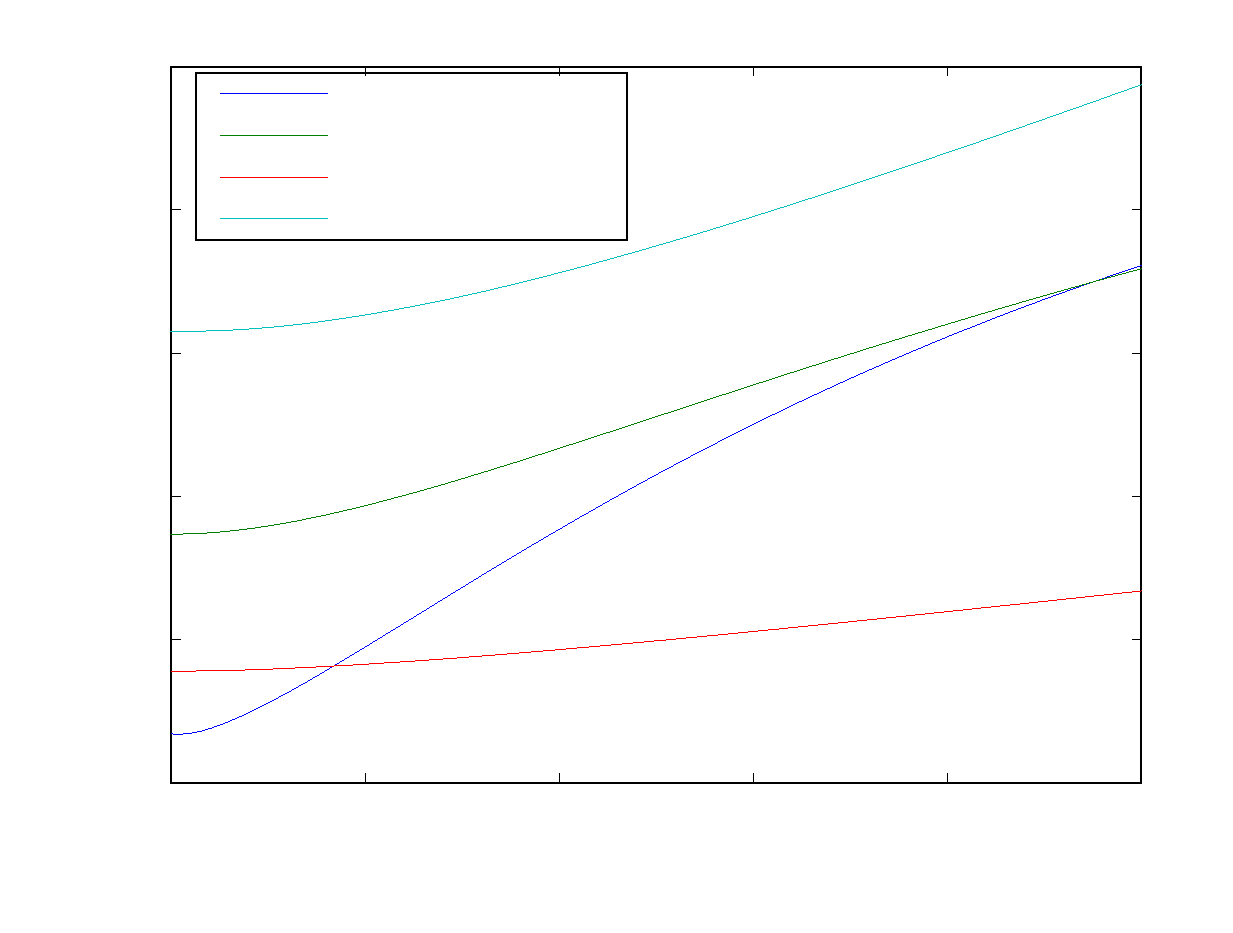
\includegraphics[width=0.6\textwidth]{chapter6/Images/MoveKurtoses.eps}
				\caption{Manipulating the Spectral Kurtoses of the Test Signals.}
				\label{fig:MoveKurtoses}
			\end{figure}

			\note{Some discussion.}

	\subsection{Tristimulus}
	\label{sec:FeatureControl-Parameterisation-Tristimulus}
		The three tristimulus metrics can be calculated using Equations \ref{eq:Tristimulus1},
		\ref{eq:Tristimulus2} and \ref{eq:Tristimulus3}.
		
		\begin{equation}
			T_{1} = \frac{h_{1}}{\sum_{n = 1}^{N} h_{n}}
			\label{eq:Tristimulus1}
		\end{equation}

		\begin{equation}
			T_{2} = \frac{h_{2} + h_{3} + h_{4}}{\sum_{n = 1}^{N} h_{n}}
			\label{eq:Tristimulus2}
		\end{equation}

		\begin{equation}
			T_{3} = \frac{\sum_{n = 5}^{N} h_{n}}{\sum_{n = 1}^{N} h_{n}}
			\label{eq:Tristimulus3}
		\end{equation}

		Where $h_{n}$ is the amplitude of the $n$\super{th} harmonic in the signal and $N$ the total number of
		harmonics.

		As mentioned in Section \ref{sec:Timbre-LowLevelFeatures-Spectral} each tristimulus metric measures the
		amplitude ratio of a specific set of harmonics and all the harmonics. In each of these equations the
		denominator is always greater than or equal to the numerator. For this reason the tristimulus takes values
		from zero to one. Zero meaning there is no energy in that set of harmonics, one meaning the signal is
		entirely composed of those harmonics.

		A generalised from of these metrics measures the amplitude ratio, $R$, of a specific set of spectral
		components, $S$, and a set which includes that set, $F$. This is shown in Equation
		\ref{eq:GeneralTristimulus}.

		\[ A = \sum_{n \in F} a_{n} \]
		\[ B = \sum_{n \in S} a_{n}, \quad S \subseteq F \]
		\begin{equation}
			R = \frac{B}{A}
			\label{eq:GeneralTristimulus}
		\end{equation}

		This ratio can be adjusted by applying gain to the spectral components in $S$. To attain a particular value
		of $R$ the required gain, $m$, can be calculated using Equation \ref{eq:GeneralTristimulusManipulation}.

		\begin{equation}
			m = \frac{R(B - A)}{B(R - 1)}, \quad 0 \leq R < 1
			\label{eq:GeneralTristimulusManipulation}
		\end{equation}

		Similar to the method discussed for controlling spectral centroid, control of tristimulus metrics involves
		altering the energy in specific bands. A reduced version of the system shown in Figure
		\ref{fig:InharmonicitySystem} can be used to control this. This system need only have individual control
		over the levels of the first four harmonics so the exciters for the fifth through ninth harmonics can be
		removed.

		\subsubsection*{Manipulation of The Tristimulus Measures}
			The first tristimulus measure is easily controlled through applying gain to the filtered
			fundamental. The other two measures can be controlled in different ways depending on the
			requirements of the system.  Individually controlling the levels of the second through fourth
			harmonics allows the second tristimulus measure to be manipulated while a more general nonlinear
			device can be used to generate higher order harmonics. As with the spectral centroid, using
			excitation to achieve this provides more flexibility as the tristimulus can be changed while
			preserving other features. For example, if the odd to even harmonic ratio needs to remain the same,
			but the second tristimulus change, different amounts of excitation can be applied to the second
			through fourth harmonics.

			Figure \ref{fig:MoveTristimulus1} shows how the first tristimuli of the test signals change when
			the gain is applied at their fundamental frequency using the system shown in Figure
			\ref{fig:InharmonicitySystem}.

			\begin{figure}[h!]
				\centering
				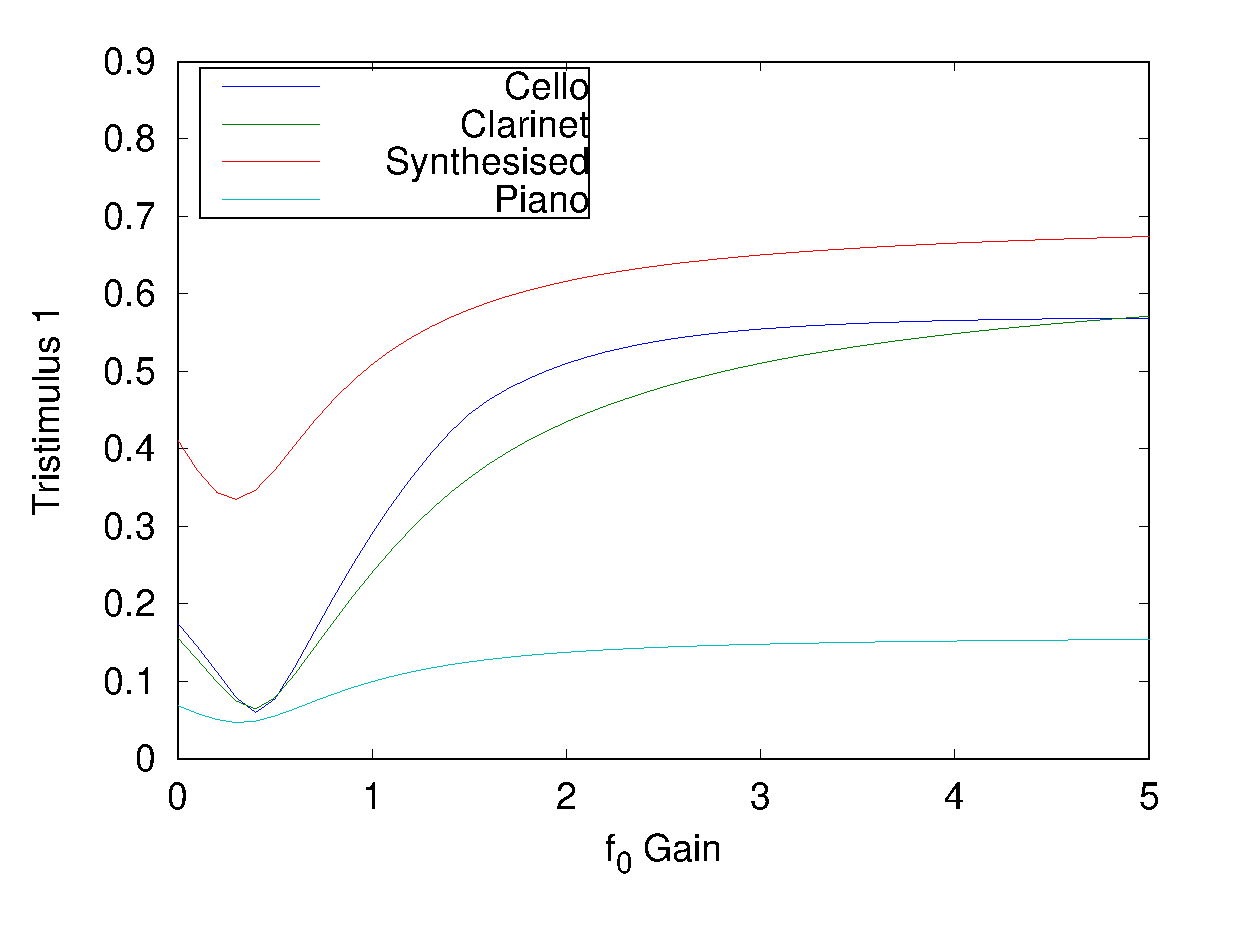
\includegraphics[width=0.6\textwidth]{chapter6/Images/MoveTristimulus1.eps}
				\caption{Manipulating the First Tristimuli of the Test Signals.}
				\label{fig:MoveTristimulus1}
			\end{figure}

			The maximum achievable first tristimulus value is determined by both the content of the input
			signal and the order of the filters used in the implementation of the excitation system. The system
			used for the values shown in Figure \ref{fig:MoveTristimulus1} used second order IIR filters. This
			means that the isolated fundamental signal contains energy in some of the higher order spectral
			partials. In sounds where the fundamental has significantly less amplitude than subsequent spectral
			partials this is particularly problematic. The piano sample used for testing illustrates this. In
			this case the isolated fundamental signal has more energy in the second harmonic than at the
			fundamental, severely reducing the maximum value which the first tristimulus can be altered to.
			Using higher order filters will alleviate this problem at the cost of increased processing.

			The order of the filters is also responsible for the initial decrease in tristimulus value with
			increasing gain. The fundamental is removed from the original signal using a high pass filter. The
			lower order this filter the more of a remnant of the fundamental remains. This initial decrease in
			the first tristimulus is due to destructive superposition between the isolated fundamental and this
			remnant. Again, increasing the order of the filters used in the system will reduce these effects.

			Control of the second tristimulus can be achieved with the same system, this time applying gain at
			to the second third and fourth excited harmonics. Figure \ref{fig:MoveTristimulus2} how the
			tristimulus value changes with increasing gain.

			\begin{figure}[h!]
				\centering
				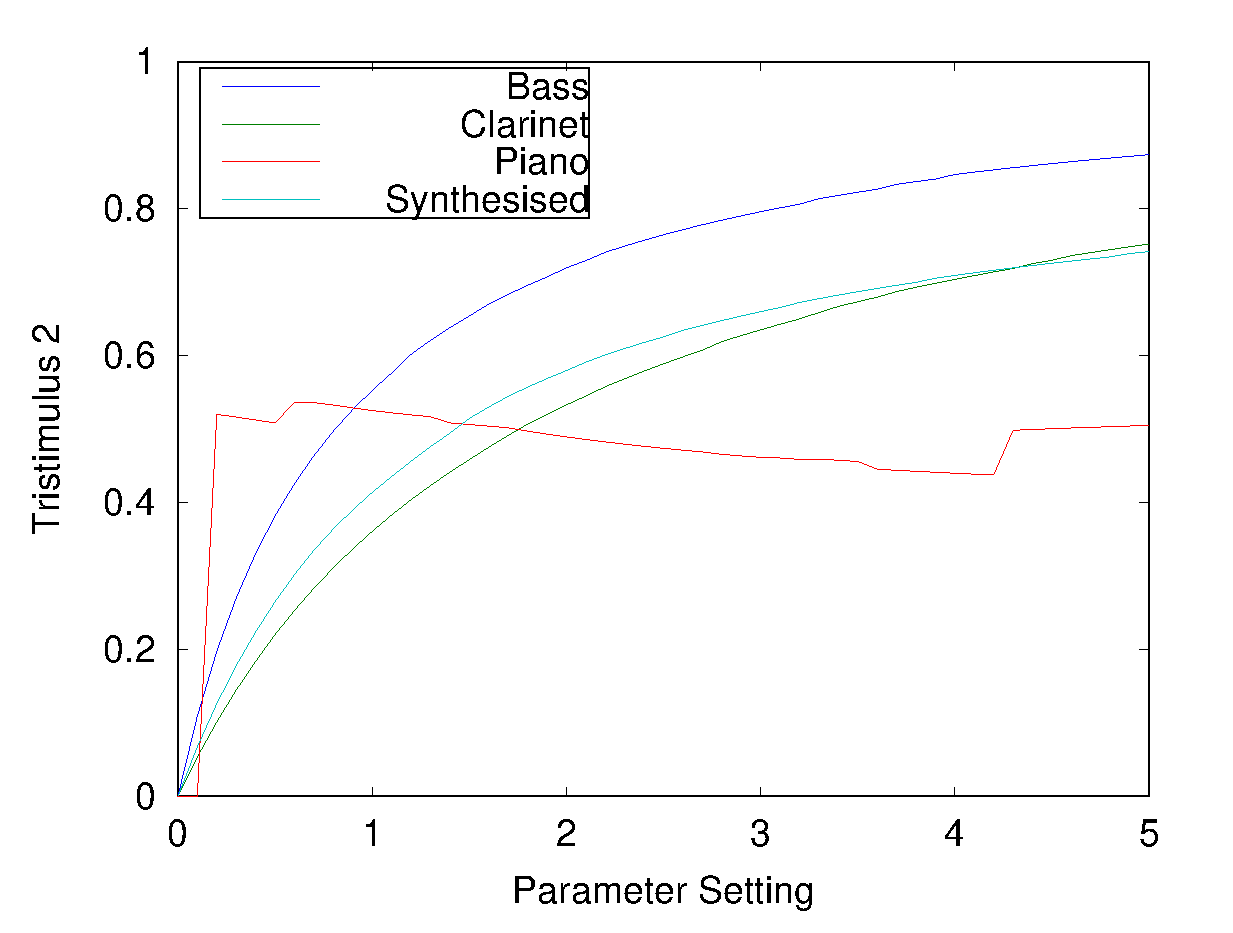
\includegraphics[width=0.6\textwidth]{chapter6/Images/MoveTristimulus2.eps}
				\caption{Manipulating the Second Tristimuli of the Test Signals.}
				\label{fig:MoveTristimulus2}
			\end{figure}

			As with control of the first tristimulus, the order of the filters used determines the maximum
			value the second tristimulus will take. The relationship is a more complex one however, as there is
			a nonlinear element to the system. The isolated fundamental signal will contain some energy at
			higher order partials.  When this signal is used to generate new harmonics some of the
			intermodulation components will be higher in frequency than the desired harmonic. This results in
			more energy being introduced above the fourth harmonic, reducing the maximum possible second
			tristimulus.

			The third tristimulus is more easily controlled using the same system as used for controlling the
			spectral centroid (Figure \ref{fig:TwoBandSpectralCentroidSystem}). A band of high order harmonics
			is generated from the isolated fundamental using a static nonlinearity and a high pass filter.
			Figure \ref{fig:MoveTristimulus3} shows how changing the gain of this band effects the third
			tristimulus of the test signals.

			\begin{figure}[h!]
				\centering
				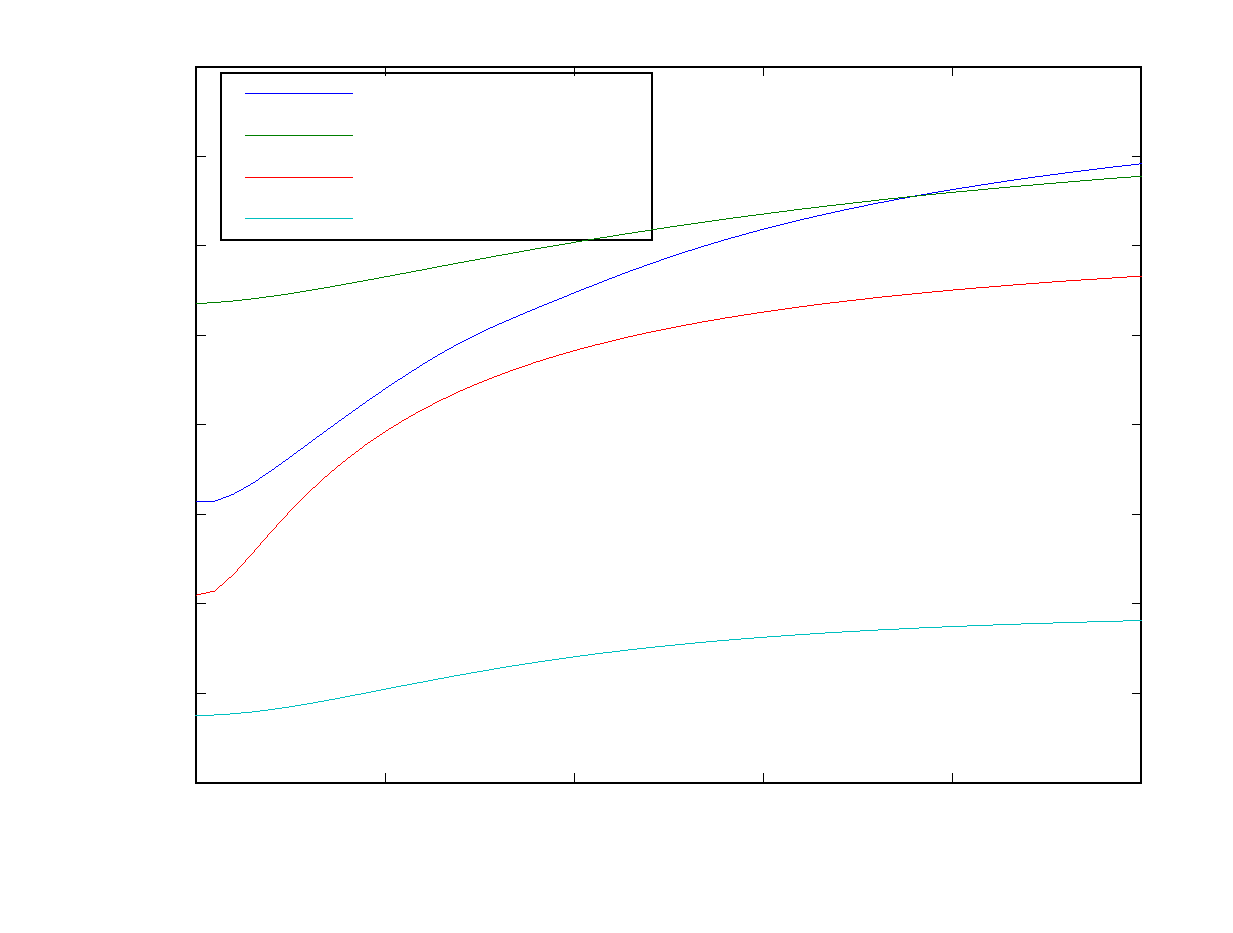
\includegraphics[width=0.6\textwidth]{chapter6/Images/MoveTristimulus3.eps}
				\caption{Manipulating the Third Tristimuli of the Test Signals.}
				\label{fig:MoveTristimulus3}
			\end{figure}

			Again, second order IIR filters have been used to filter out the lower order harmonics from the
			excited signal.	These low order filters do not remove all the energy in the first 4 harmonics
			thereby limiting how high the third tristimulus can be made.

	\subsection{Odd to Even Harmonic Ratio}
	\label{sec:FeatureControl-Parameterisation-HarmonicParityRatio}
		The odd to even order harmonics ratio is calculated using Equation \ref{eq:HarmonicParityRatio}.
		
		\begin{equation}
			R_{\textrm{OE}} = \frac{\sum_{1 \leq n \leq N, n \textrm{ is odd}} h_{n}^{2}}
			              {\sum_{1 \leq n \leq N, n \textrm{ is even}} h_{n}^{2}}
			\label{eq:HarmonicParityRatio}
		\end{equation}

		It describes how much of the signals energy is made up of odd or even order harmonics. This allows for
		distinction between signal which consist only of odd harmonics or of even harmonics. The ration can easily
		be altered by applying gain to the odd harmonics. The required gain factor, $m$, is calculated using
		Equation \ref{eq:HarmonicParityRatioManipulation}.

		\begin{equation}
			m = \sqrt{\frac{R_{\textrm{OE}}\sum_{1 \leq n \leq N, n \textrm{ is even}} h_{n}^{2}}
			               {\sum_{1 \leq n \leq N, n \textrm{ is odd}} h_{n}^{2}}},
				       \quad R_{\textrm{OE}} \geq 0;
		       \label{eq:HarmonicParityRatioManipulation}
		\end{equation}

		Equation \ref{eq:HarmonicParityRatio} produces an asymmetric scale which may be difficult to interpret.
		Signals with most of their energy at even harmonics produce values between zero and one. Signals with more
		energy at the odd harmonics can produce any value greater then one. Another problem arises for signals with
		no energy at even harmonics where a division by zero will occur.

		A more robust measure is to have separate measures for the proportion of odd harmonics in a signal and the
		proportion of even harmonics in a signal.  \citet{lukasik2005towards} describes two metrics which measure
		the oddness, $O$, and the evenness, $E$, of a signal. These are given in Equations \ref{eq:Oddness} and
		\ref{eq:Evenness}.

		\begin{equation}
			O = \sqrt{\frac{\sum_{1 \leq n \leq N, n \textrm{ is odd}} h_{n}^{2}}
			               {\sum_{n = 1}^{N} h_{n}^{2}}}
			\label{eq:Oddness}
		\end{equation}

		\begin{equation}
			E = \sqrt{\frac{\sum_{1 \leq n \leq N, n \textrm{ is even}} h_{n}^{2}}
			               {\sum_{n = 1}^{N} h_{n}^{2}}}
			\label{eq:Evenness}
		\end{equation}

		These both produce values in the range zero to one and satisfy the statement $O + E = 1$. 

		Equations \ref{eq:Oddness} and \ref{eq:Evenness} can be generalised to give Equation
		\ref{eq:GeneralOddness}.

		\[ A = \sum_{n \in F} a_{n}^{2} \]
		\[ B = \sum_{n \in S} a_{n}^{2}, \quad S \subseteq F \]
		\begin{equation}
			R = \sqrt{\frac{B}{A}}
			\label{eq:GeneralOddness}
		\end{equation}

		Like Equation \ref{eq:GeneralTristimulus} this measures the ratio of amplitudes of a set of frequencies and
		a larger set of frequencies. This time using the squares of the amplitudes and taking the square root
		afterwards. The value of the ratio can be altered by applying gain to the spectral components in the set
		$S$. The required gain factor, $m$, is calculated using Equation \ref{eq:GeneralOddnessManipulation}.

		\begin{equation}
			m = \sqrt{\frac{R^{2}(B - A)}{B(R^{2} - 1)}}, \quad 0 \leq R < 1
			\label{eq:GeneralOddnessManipulation}
		\end{equation}

		\subsubsection*{Manipulation of Odd to Even Harmonic Ratio}
			For control over the oddness or evenness of a signal a system which provides control over
			individual harmonics is not necessary. While this level of control allows for more complex
			manipulations a simpler system can be employed if only the oddness and evenness are to be changed.
			Such a system is shown in Figure \ref{fig:HarmonicParitySystem}.

			\begin{figure}[h!]
				\centering
				\begin{tikzpicture}
					\node (In) at (-1, -2.25) {$x[n]$};
					\coordinate (InMid) at (0, -2.25);
					\draw (In) -- (InMid);

					\coordinate (Side) at (0, -1.25);
					\draw (InMid) -- (Side);

					\node (F0) [draw] at (2, -1.25) {Fundamental Tracker};
					\node (F0Filter) [draw] at (2, -2.25) {LPF};
					\draw (InMid) -- (F0Filter);
					\draw (F0) -- (F0Filter);
					\draw (Side) -- (F0);

					\node (Add) [operator] at (11.5, -2.25) {+};

					\coordinate (ExciterIn) at (4, -2.25);
					\draw (F0Filter) -- (ExciterIn);

					% odd harmonics
					\coordinate (OddIn) at (4, -1.25);
					\node (Odd) [draw] at (6, -1.25) {Odd Harmonics};
					\draw (OddIn) -- (Odd);

					\node (OddFilter) [draw] at (8.5, -1.25) {Filter};
					\draw (Odd) -- (OddFilter);

					\node (OddGain) [gain] at (10, -1.25) {};
					\draw (OddFilter) -- (OddGain);
					\coordinate (OddOut) at (10.5, -1.25);
					\draw (OddGain) -- (OddOut);
					\draw (OddOut) -- (Add);

					% even harmonics
					\coordinate (EvenIn) at (4, -2.25);
					\draw (OddIn) -- (EvenIn);
					\node (Even) [draw] at (6, -2.25) {Even Harmonics};
					\draw (EvenIn) -- (Even);

					\node (EvenFilter) [draw] at (8.5, -2.25) {Filter};
					\draw (Even) -- (EvenFilter);

					\node (EvenGain) [gain] at (10, -2.25) {};
					\draw (EvenFilter) -- (EvenGain);
					\coordinate (EvenOut) at (10.5, -2.25);
					\draw (EvenGain) -- (EvenOut);
					\draw (EvenOut) -- (Add);

					% through
					\coordinate (Through) at (0, -3.25);
					\draw (InMid) -- (Through);
					\node (ThroughFilter) [draw] at (8.5, -3.25) {Filter};
					\draw (Through) -- (ThroughFilter);
					\node (ThroughGain) [gain] at (10, -3.25) {};
					\draw (ThroughFilter) -- (ThroughGain);
					\coordinate (ThroughOut) at (10.5, -3.25);
					\draw (ThroughGain) -- (ThroughOut);
					\draw (ThroughOut) -- (Add);

					\node (Out) at (12.5, -2.25) {$y[n]$};
					\draw (Add) -- (Out);
				\end{tikzpicture}
				\caption{A system to control the levels of odd and even order harmonics individually.}
				\label{fig:HarmonicParitySystem}
			\end{figure}

			This system uses two parallel static nonlinearities to generate two signals consisting of only odd
			harmonics and even harmonics respectively. The properties of these nonlinearities can be adjusted
			to shape the spectra of each of these signals which are further shaped through linear filtering.
			The gains of these two signals allow control over the oddness and evenness of the signal using
			Equation \ref{eq:GeneralOddnessManipulation}.

			The odd and even harmonics in a signal could be separated using linear filters. This approach
			requires in depth analysis of the signal adding complexity and possible delay to the system but has
			some advantage in preservation of signal characteristics. When using excitation this complexity is
			reduced but the problems discussed in Section \ref{sec:FeatureControl-Systems-Superposition} become
			apparent. To elicit full control over the levels of the odd and even harmonics using the system
			shown in Figure \ref{fig:HarmonicParitySystem} all the harmonic content in the output signal is
			generated by the nonlinearities. This is likely to cause a dramatic change in timbre as most of the
			information present in the original signal has been replaced. 

			A method to counteract this is to only excite even or odd harmonics in the signal at any one time.
			The relative levels of odd and even harmonics can still be adjusted but some more of the original
			signals spectral shape is preserved. Avoiding superposition still remains difficult in this
			situation as it would mean filtering out alternate harmonics in the input signal. Allowing
			superposition to occur sacrifices accurate control in order to maintain some of the input's
			characteristics.

			An example of how the system in Figure \ref{fig:HarmonicParitySystem} can be used is as follows.
			The isolated fundamental of each test signal id processed with both even and odd hard clipping
			functions to generate separate bands of each parity of harmonic. Each band of harmonics is then low
			passed filtered with a cutoff at the frequency of the ninth harmonic and the original signal is
			high pass filtered at the same frequency. The ninth harmonic is chosen due to it being the highest
			individually resolved harmonic as discussed in Section
			\ref{sec:FeatureControl-Systems-SpectralShaping}. The three signals are then summed at different
			ratios to control the evenness or oddness of the output. Figure \ref{fig:MoveParities} shows the
			effects of manipulating the levels of odd and even order harmonics in this way. The original signal
			remains at unity gain whereas the gains of the harmonic bands are determined by a parameter, $P$.
			Odd order harmonics are multiplied by a gain of $P$ and even order harmonics by $1 - P$.

			\begin{figure}[h!]
				\centering
				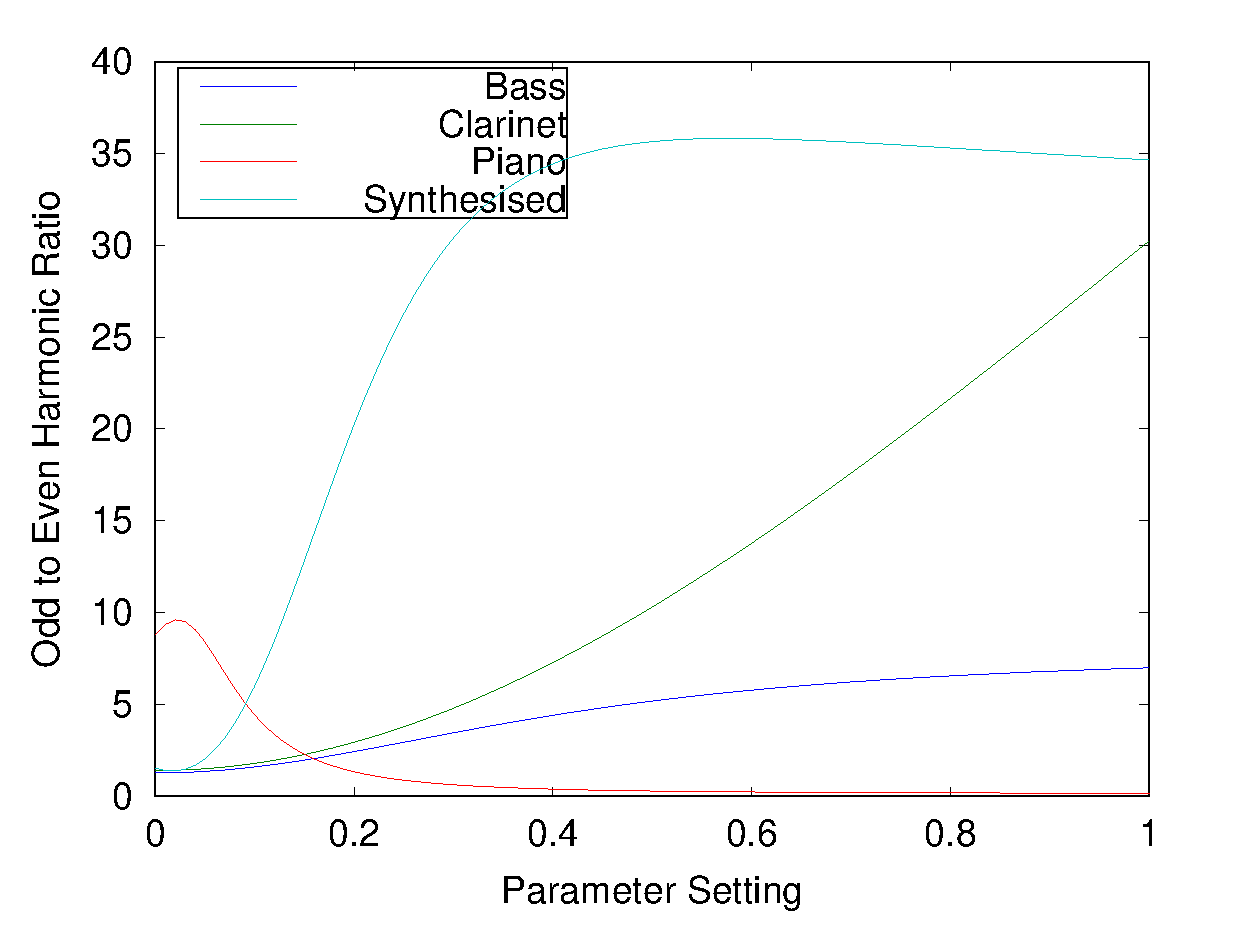
\includegraphics[width=0.6\textwidth]{chapter6/Images/MoveParities.eps}
				\caption{Manipulating the Odd to Even Harmonic Ratios of the Test Signals.}
				\label{fig:MoveParities}
			\end{figure}

			Here we see how the spectral content of the input signal influences the effects of the processing.
			The $R_{\textrm{OE}}$ of the clarinet signal seems to be the easiest to control. This can be
			attributed to the high oddness of the unprocessed clarinet signal, the fundamental easier to
			isolate because there is very little energy in the second harmonic. With a better isolated
			fundamental the two bands of excited harmonics will be better separated with respect to the
			parities of harmonics they contain.

			The bass and synthesised samples both exhibit a limit on how high the $R_{\textrm{OE}}$ can be
			made. This is due to both bands of excited harmonics containing both parities of harmonic.  The
			general upward trend for both samples illustrates that the two bands generated do contain the
			majority of their energy in the correct parity harmonics but higher order filtering of the
			fundamental is needed to better segregate them. The decrease in $R_{\textrm{OE}}$ seen for the
			synthesised signal is due to destructive superposition between the harmonics in the three signals
			being summed.

			The system discussed here provides no control over the $R_{\textrm{OE}}$ of the piano sample. This
			is again due to the low amplitude fundamental. The isolated fundamental signal contains the
			majority of its energy in the second harmonic. This causes the two bands of generated harmonics to
			both contain mostly even order harmonics, meaning the resulting signal will have a high evenness,
			or low $R_{\textrm{OE}}$.

	\subsection{Inharmonicity}
	\label{sec:FeatureControl-Parameterisation-Inharmonicity}
		Inharmonicity is a measure of how much the frequencies of a signal's partials deviate from harmonic
		frequencies. This is measured using Equation \ref{eq:Inharmonicity}.
		
		\begin{equation}
			I = \frac{2\sum_{n = 1}^{N}a_{n}^{2}
			           \abs{\nu_{n} - f_{0}\floor{\frac{\nu_{n}}{f_{0}} + \frac{1}{2}}}}
				   {f_{0}\sum_{n = 1}^{N} a_{n}^{2}}
			\label{eq:Inharmonicity}
		\end{equation}

		Where $a_{n}$ and $\nu_{n}$ are the amplitude and frequency of the $n$\super{th} partial in the signal
		respectively and $N$ the total number of partials in the signal.

		This produces values between zero and one. Zero describing a signal in which all partials are harmonics of
		the fundamental and one describing a signal where all partials have frequencies lying
		$\frac{f_{0}}{2}$Hz from harmonic frequencies.

%		Controlling the inharmonicity can prove difficult unless certain criteria are met. Consider two signals,
%		$x$ and $y$, with the same fundamental frequency, which are composed of partials with frequencies in the
%		sets $X$ and $Y$ respectively. Provided that $X \medcap Y = \emptyset$ (i.e. $x$ and $y$ have no frequency
%		component in common) the inharmonicity of $x + y$ is given by Equation \ref{eq:InharmonicitySum}.
%
%		\begin{equation}
%			I = \frac{I_{x}\sum_{\nu \in X} a_{\nu,x}^{2} + I_{y}\sum_{\nu \in Y} a_{\nu,y}^{2}}
%			         {\sum_{\nu \in X} a_{\nu,x}^{2} + \sum_{\nu \in Y} a_{\nu,y}^{2}}
%			\label{eq:InharmonicitySum}
%		\end{equation}
%
%		Where $a_{\nu,x}$ and $a_{\nu,y}$ are the amplitudes of frequency $\nu$ in signals $x$ and $y$, and $I_{x}$
%		and $I_{y}$ are the inharmonicities of signals $x$ and $y$.
%
%		The inharmonicity of the sum of the signals can be altered by changing the relative amplitudes of the
%		signals. To produce a given inharmonicity, $I$, when summing two signals, $x$ and $y$, which have no
%		frequency components in common, a gain factor $m$, calculated using Equation
%		\ref{eq:InharmonicityManipulation}, can be applied to signal $x$.  Note that the target inharmonicity must
%		lie between the inharmonicities of the two signals being summed.
%
%		\begin{equation}
%			m = \sqrt{\frac{(I_{y} - I)\sum_{\nu \in Y} a_{\nu,y}^{2}}
%			               {(I - I_{x})\sum_{\nu \in X} a_{\nu,x}^{2}}},
%			\quad I_{x} \leq I < I_{y} \quad \textrm{or} \quad I_{y} < I \leq I_{x}
%			\label{eq:InharmonicityManipulation}
%		\end{equation}

		\subsubsection*{Manipulation of Inharmonicity}
			While it is reasonably simple to introduce inharmonicity in harmonic excitation systems,
			controlling the inharmonicity of a signal is a more complicated problem. The system shown in Figure
			\ref{fig:InharmonicitySystem} can be use to apply multiple approaches approach to this problem. 

%			Equation \ref{eq:InharmonicitySum} allows the inharmonicity of the sum of two signals to be
%			calculated, provided the signals have the same fundamental and share no frequency content. This
%			allows us to adjust the relative gains of two signals to control the resulting inharmonicity. The
%			problematic task is how to construct these two signals.
			
			A simple two band system leaves the lower partials of the system unaltered and generates a high
			band using a static nonlinearity and filtering. The inharmonicities in this high band will be
			amplified versions of those in the original signal. This approach is not applicable in a number of
			situations such as when the input only contains perfectly harmonic partials or when the desired
			result is a signal with reduced inharmonicity.
			
			The inverse system, in which the high frequencies are left unaltered and the low frequency partials
			are generated individually, provides a greater amount of control over the inharmonicity of the
			resulting signal. The newly generated partials can be put at frequencies closer to harmonics than
			the originals reducing the overall inharmonicity. It also allows for generation of inharmonic
			partials in a signal with zero inharmonicity. 

			This system is more complicated both in computation and use. Because the inharmonicity metric
			(Equation \ref{eq:Inharmonicity}) depends on the frequencies of every partial, there are numerous
			ways a signal can be manipulated resulting in the same value for the inharmonicity. When
			manipulating the inharmonicity a decision needs to be made as to which partials are to be made
			inharmonic and by how much. One method of deciding this is to model it on the vibrational modes of
			an acoustic instrument, ensuring a natural set of inharmonic partials. To increase the
			inharmonicity the frequencies of the partials can be moved from being harmonic towards the
			frequencies indicated by the model.

			One such model is that given by \citet{rossing2002the} for calculating the frequencies of the
			spectral partials of piano strings. In this model the frequencies of each partial are determined by
			an inharmonicity factor, $A$, using Equation \ref{eq:PianoInharmonicity}. In the modelling of piano
			timbre the value of $A$ is calculated from the physical properties of the piano string. For
			creative purposes the value of $A$ can be arbitrarily set.

			\begin{equation}
				a_{n} = nf_{0} \left( 1 + \left( n^{2} - 1 \right) A \right);
				\label{eq:PianoInharmonicity}
			\end{equation}

			Using the system shown in Figure \ref{fig:InharmonicitySystem} the inharmonicities of the first
			nine harmonics of a signal can be set according to this model. Figure \ref{fig:MoveInharmonicities}
			shows how the resulting inharmonicity changes with the inharmonicity factor $A$.

			\begin{figure}[h!]
				\centering
				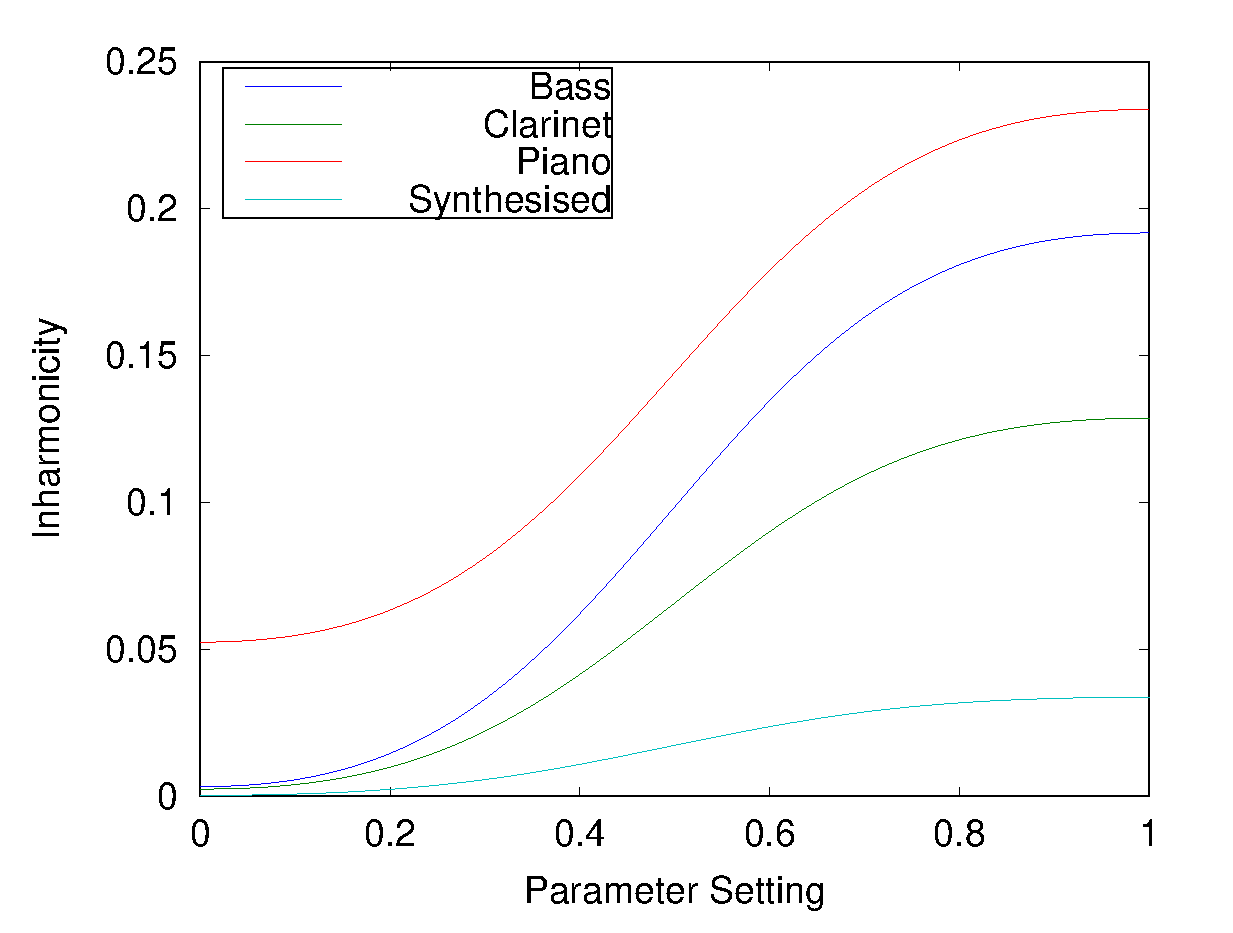
\includegraphics[width=0.6\textwidth]{chapter6/Images/MoveInharmonicities.eps}
				\caption{Manipulating the Inharmonicities of the Test Signals.}
				\label{fig:MoveInharmonicities}
			\end{figure}

			As only the first nine harmonics are being altered, the degree to which the inharmonicity can be
			manipulated depends on the spectral content of the input signal. In the synthesised sample all of
			the spectral partials are at perfectly harmonic frequencies and there is significant energy in the
			harmonics with higher order than the ninth. The inharmonic signal generated from the synthesised
			sample then still has a significant amount of energy in perfectly harmonic partials giving it a low
			inharmonicity. This reduces the range of values which the resulting inharmonicity can take. The
			other three samples all have higher spectral roll off, such that the influence of their existing
			high order partials has a smaller effect on the overall inharmonicity.

			The issue of higher order harmonics reducing the maximum inharmonicity could be counteracted by
			adding an addition frequency shifter to the system. This shifter would operate on the filtered
			input signal and shift all the higher order partials by the same amount.

	\subsection{Spectral Irregularity}
	\label{sec:FeatureControl-Parameterisation-Irregularity}
		Spectral irregularity measures the smoothness of a spectrum. Various different methods of measuring this
		are often cited in the literature. The first being that proposed by \citet{krimphoff1994caracterisation},
		shown in Equation \ref{eq:KrimphoffIrregularity}.

		\begin{equation}
			\textrm{KI} = \log \left( 20 \sum_{n = 2}^{N - 1}
				                  \abs{\log(a_{n}) - \frac{\log(a_{n-1}a_{n}a_{n+1})}{3}}
					   \right)
			\label{eq:KrimphoffIrregularity}
		\end{equation}

		This is often implemented using the magnitude of the raw amplitude rather than their dB amplitude yielding
		equation \ref{eq:LibXtractKrimphoffIrregularity}. This is how the Krimphoff irregularity is implemented
		in LibXtract \citep{bullock2007libxtract}, and in the SAFE plug-ins.

		\begin{equation}
			\textrm{KI} = \sum_{n = 2}^{N - 1}
					  \abs{a_{n} - \frac{a_{n-1} + a_{n} + a_{n+1}}{3}}
			\label{eq:LibXtractKrimphoffIrregularity}
		\end{equation}
		

		A second method is proposed by \citet{jensen1999timbre}, shown in Equation \ref{eq:JensenIrregularity}.

		\begin{equation}
			\textrm{JI} = \frac{\sum_{n = 1}^{N} (a_{n} - a_{n+1})^{2}}
			                   {\sum_{n = 1}^{N} a_{n}^{2}},
			              \quad a_{N+1} = 0
			\label{eq:JensenIrregularity}
		\end{equation}

		A third method is given by \citet{beauchamp2007analysis}, shown in Equation \ref{eq:BeauchampIrregularity}.

		\[ \bar{a}_{n} = \frac{a_{n-1} + a_{n} + a_{n+1}}{3} \]
		\begin{equation}
			\textrm{BI} = \frac{\sum_{n = 2}^{N - 1} \bar{a}_{n} \abs{a_{n} - \bar{a}_{n}}}
					   {\sum_{n = 2}^{N - 1} \bar{a}_{n} \sqrt{\sum_{n = 1}^{N} a_{n}^{2}}}
			\label{eq:BeauchampIrregularity}
		\end{equation}

		Equation \ref{eq:JensenIrregularity} and \ref{eq:BeauchampIrregularity} have an advantage over Equations
		\ref{eq:KrimphoffIrregularity} and \ref{eq:LibXtractKrimphoffIrregularity} in that they produce normalised
		values. Equation \ref{eq:JensenIrregularity} produces values between zero and two while Equation
		\ref{eq:BeauchampIrregularity} produces values between zero and one. This allows measures of irregularity
		of two different signals to be compared more easily.

		\subsubsection*{Manipulation of Irregularity}
			\citet{beauchamp2007analysis} proposes methods for manipulating the spectral irregularity in
			additive synthesis systems. In effect these involve filtering of the frequency domain
			representation of a signal, applying a filter to the amplitudes of the signals spectral components.
			This does not allow the irregularity to be set to a precise value but gives control over the
			direction in which the irregularity will change. Low pass filtering the spectral components'
			amplitudes will decrease the irregularity while a high pass filter will do the opposite.
			
			Both the Krimphoff and Beauchamp irregularities (Equations \ref{eq:KrimphoffIrregularity} and
			\ref{eq:BeauchampIrregularity}) are based on taking the differences between each partial's
			amplitude and the mean amplitude of itself and the two partials surrounding it. Intuitively this
			value can be increased or reduced by moving the amplitudes of the partials away or towards their
			mean. To implement this using the system shown in Figure \ref{fig:InharmonicitySystem} the new
			amplitudes of the first nine harmonics can be calculated using Equation \ref{eq:PartialSmoothing}
			
			\note
			{
				This is bad and needs redoing. It will end up with negative amplitudes.
			}

			\begin{equation}
				a'_{n} = a_{n} - P \left(a_{n} - \sum_{k = 1}^{9} a_{k} \right)
				\label{eq:PartialSmoothing}
			\end{equation}

			Where $a'_{n}$ is the new amplitude of the $n$\super{th} partial, $a_{n}$ is the amplitude of the
			$n$\super{th} partial in the input signal and $P$ is a parameter. Figure
			\ref{fig:MoveIrregularities} shows how each of the spectral irregularity measures is affected by
			changes in the value of $P$.

			\begin{figure}[h!]
				\centering
				\subfloat[Krimphoff Irregularity]
				{
					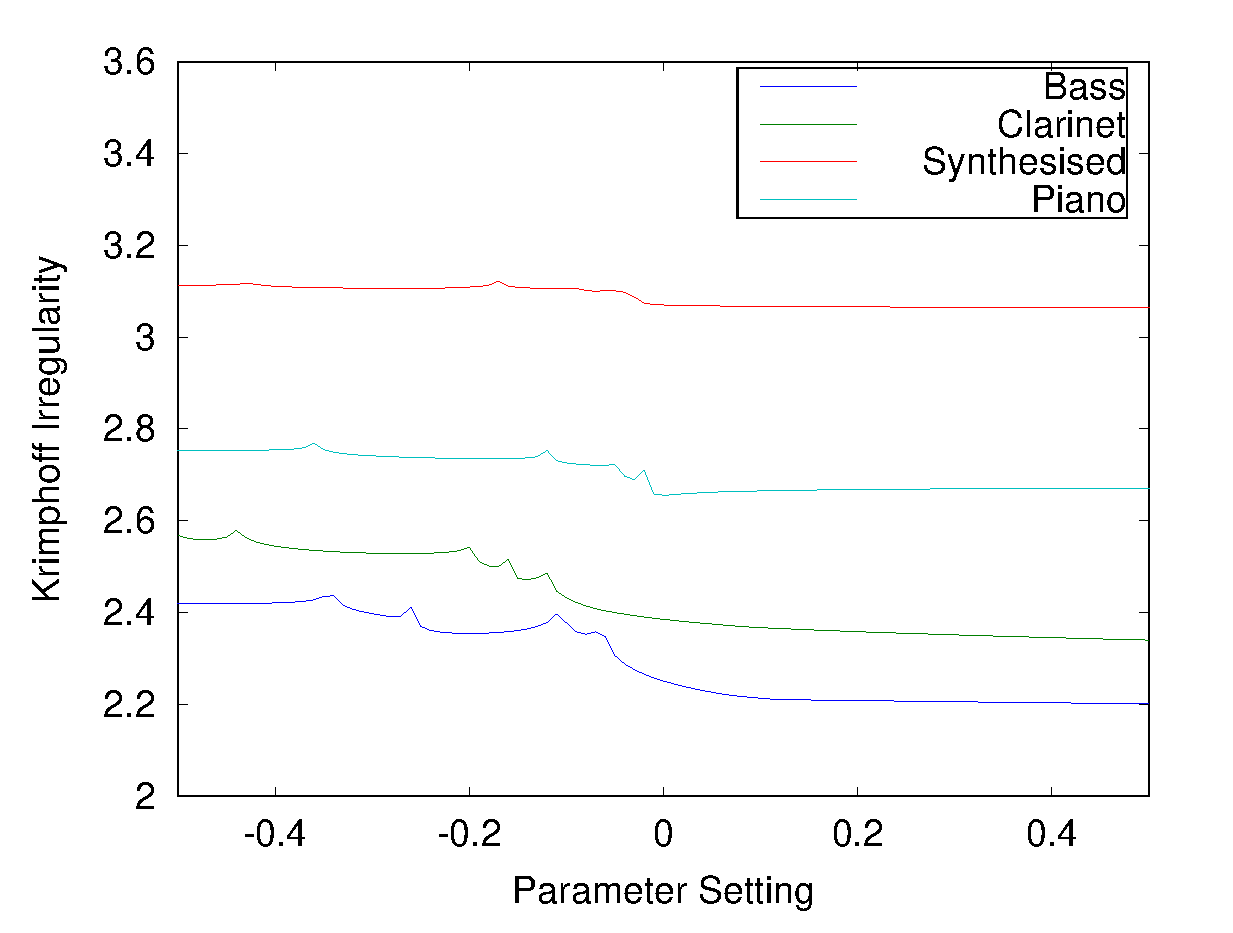
\includegraphics[width=0.45\textwidth]{chapter6/Images/MoveIrregularitiesK.eps}
					\label{fig:MoveIrregularitiesK}
				}
				\qquad
				\subfloat[Jensen Irregularity]
				{
					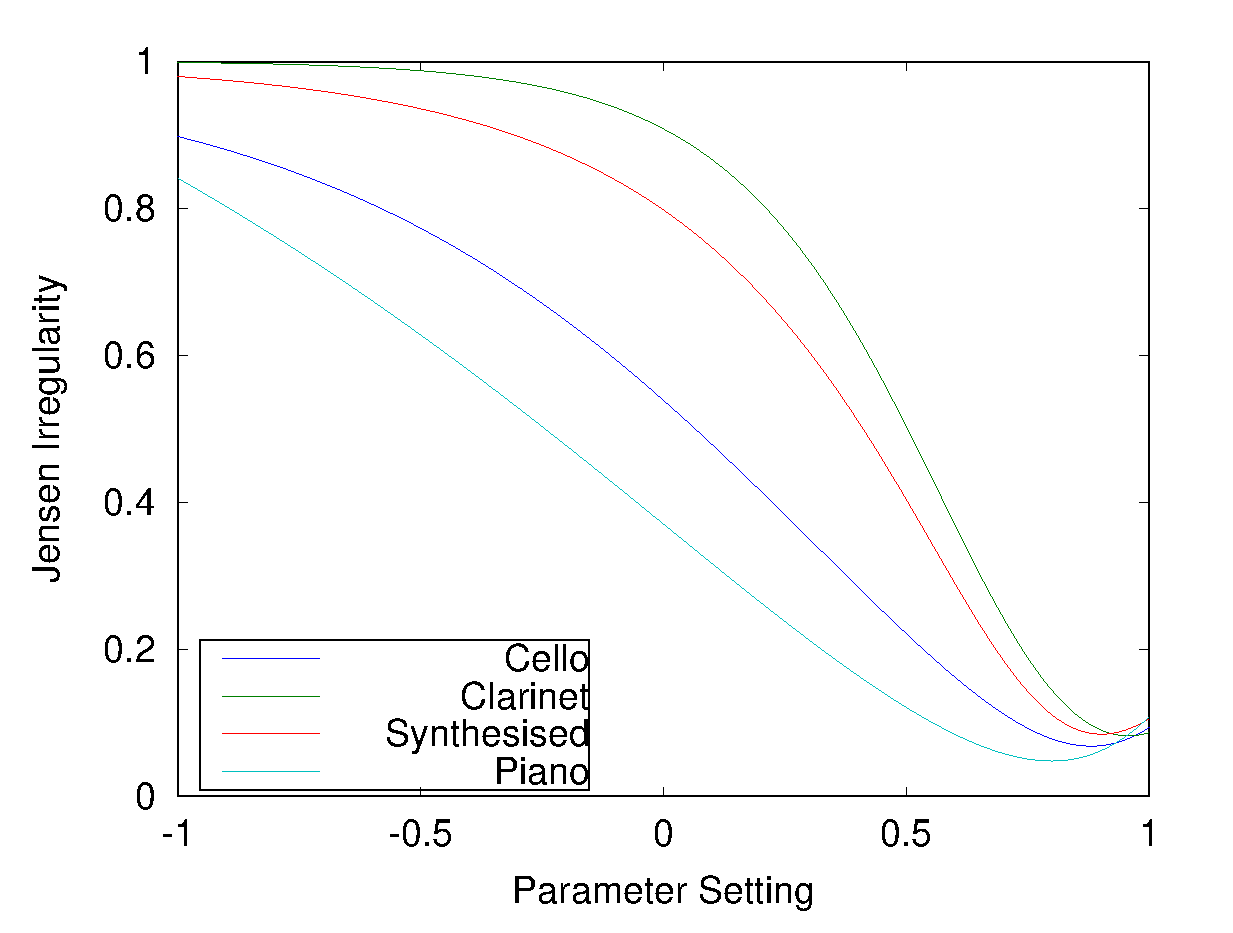
\includegraphics[width=0.45\textwidth]{chapter6/Images/MoveIrregularitiesJ.eps}
					\label{fig:MoveIrregularitiesJ}
				}
				
				\subfloat[Beauchamp Irregularity]
				{
					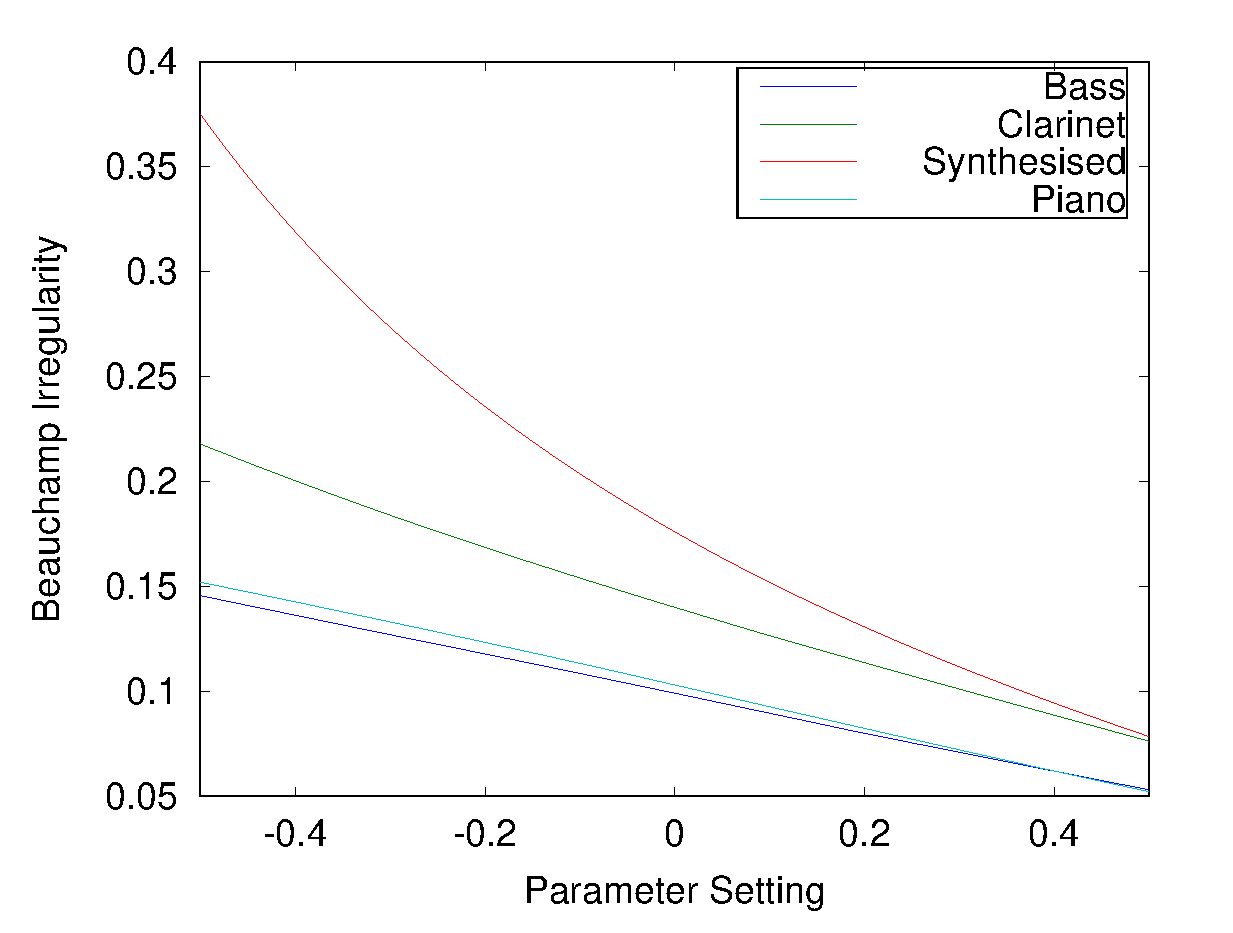
\includegraphics[width=0.45\textwidth]{chapter6/Images/MoveIrregularitiesB.eps}
					\label{fig:MoveIrregularitiesB}
				}
				\caption{Manipulating the Spectral Irregularities of the Test Signals.}
				\label{fig:MoveIrregularities}
			\end{figure}

			This method provides effective control over both the Jensen and Beauchamp irregularities (Equations
			\ref{eq:JensenIrregularity} and \ref{eq:BeauchampIrregularity}). The Krimphoff irregularity
			(Equation \ref{eq:KrimphoffIrregulatiry}) however, is not as 

			Achieving this using excitation requires an analysis and resynthesis approach, replacing the
			existing spectral components with excited ones and chaining the amplitudes to give the desired
			irregularity.  If the analysis stage is removed the complexity of the system can be greatly
			reduced. The amplitudes of the newly excited spectral components can be predetermined and the
			irregularity manipulated through filtering as before. A different number of spectral components can
			be replaced with excited ones depending on how large a timbral variation is desired. Replacing only
			a few spectral components will provide a small amount of control over irregularity while preserving
			most of the spectrum of the input signal. Replacing more spectral components provides more control
			over the overall irregularity at the cost of losing spectral information from the original.

			An alternate way to influence the irregularity of a signal is through control of the oddness and
			evenness as discussed in Section \ref{sec:FeatureControl-Parameterisation-HarmonicParityRatio}. A
			signal with a high oddness and low evenness (or vice versa) will have a high a spectral
			irregularity whereas a signal with a more even distribution of energy between odd and even
			harmonics will have a lower irregularity. This allows the irregularity of a signal which contains
			both parities of harmonics can be changed by altering the signals oddness or evenness.

	\subsection{Spectral Flatness}
	\label{sec:FeatureControl-Parameterisation-Flatness}
		Spectral flatness measures how uniformly distributed the energy is in the spectrum.
		\citet{johnston1988transform} measures the spectral flatness as the ratio of the geometric and arithmetic
		means of the power spectrum of a signal (Equation \ref{eq:Flatness}).

		\begin{equation}
			\textrm{SF} = \frac{N\sqrt[N]{\prod_{n = 1}^{N} a_{n}^{2}}}
				           {\sum_{n = 1}^{N} a_{n}^{2}}
			\label{eq:Flatness}
		\end{equation}

		The arithmetic and geometric means of any list of $N$ non-negative numbers, $L$, satisfy the inequality in
		Equation \ref{eq:MeanInequality}.

		\begin{equation}
			\sqrt[N]{\prod_{n = 1}^{N} L_{n}} \leq \frac{1}{N} \sum_{n = 1}^{N} L_{n}
			\label{eq:MeanInequality}
		\end{equation}

		Where $L_{n}$ is the $n$\super{th} element of list $L$. The two means are only equal if all elements of $L$
		have the same value.

		Due to this the spectral flatness of a signal takes a value between zero and one. Low values describe
		signals whose energy lies in narrow bands of the spectrum (tones). High values describe signals whose
		energy is more spread out, a value of one describing a signal where all bins of the power spectrum have the
		same amplitude (white noise). This means the spectral flatness also gives a description of the tonality /
		noisiness of a signal.

		The spectral flatness is traditionally measured using DFT bins as spectral components. This way any signal
		which has zero energy in any DFT bin will produce a spectral flatness of zero. Musical signals which are
		composed of a set of frequency partials may have areas of the spectrum with zero energy. Several different
		sounds with radically different spectral envelopes can then all exhibit a spectral flatness of zero. This
		is particularly problematic for digitally synthesised signals as they do not have the inherent noise
		present in recorded sounds. The method used by \citet{peeters2004a} mitigates this by using frequency bands
		as the spectral components. It is less likely that there will be zero energy in a wider spectral band than
		a single DFT bin. 
		
		Another method to avoid spectral flatnesses of zero is to use the signals partials as spectral components.
		This no longer measures the tonality / noisiness of a signal but rather the flatness of its spectral
		envelope.

		\subsubsection*{Manipulation Of Spectral Flatness}
			Spectral flatness is related to spectral irregularity. Many of the techniques to reduce the
			irregularity will also increase the flatness. More precisely any manipulation which moves the
			amplitudes of all spectral components closer to each other will increase the spectral flatness. To
			take an example from Section \ref{sec:FeatureControl-Parameterisation-Irregularity}, using a low
			pass filter on the amplitudes of the spectral components will increase the flatness of the
			spectrum.

			A greater degree of control can be achieved over the spectral flatness by altering the power
			spectrum such that one of the means changes while the other remains the same. The method discussed
			here changes the arithmetic mean but preserves the geometric mean. 

			Consider two disjoint sets, $L$ and $H$, which are each composed of the indices of $k$ spectral
			components of the signal such that the total energy in the spectral components denoted by $L$ is
			less than that of the spectral components denoted by $H$. A gain $m$ is applied to the spectral
			components denoted by set $H$ and the reciprocal gain $\frac{1}{m}$ applied to the spectral
			components denoted by set $L$. The resulting spectral flatness is calculated using Equation
			\ref{eq:FlatnessManipulation}.

			\[ P = \left\{ n | n \in \textbf{N} \land n \leq N \right\} \]
			\[ E = P \setminus (L \medcup H) \]
			\[ A_{L} = \sum_{n \in L} a_{n}^{2} \quad A_{H} = \sum_{n \in H} a_{n}^{2}
			   \quad A_{E} = \sum_{n \in E} a_{n}^{2} \]
			\begin{equation}
				\textrm{SF} = \frac{N\sqrt[N]{\prod_{n \in P} a_{n}^{2}}}
						   {\frac{A_{L}}{m^{2}} + m^{2}A_{H} + A_{E}}
				\label{eq:FlatnessManipulation}
			\end{equation}

			The spectral flatness can be increased by using a value of $m$ such that
			$\sqrt{\frac{A_{L}}{A_{H}}} < m < 1$. The maximum possible flatness which can be achieved with the
			selected spectral components occurs when $m = \sqrt[4]{\frac{A_{L}}{A_{H}}}$. To decrease the
			spectral flatness a value of $m$ satisfying $0 < m < \sqrt{\frac{A_{L}}{A_{H}}}$ or $m > 1$ should
			be used. When $m = \sqrt{\frac{A_{L}}{A_{H}}}$ the arithmetic mean is unchanged, this provides a
			point at which the energy has been redistributed in the spectrum but the spectral flatness remains
			the same. 

			The gain value, $m$, can be calculated from a simplified control parameter, $P$, using Equation
			\ref{eq:FlatnessControlParameter}. When $P$ is equal to 0 or 1 the spectral flatness will be
			unchanged. Values of $P$ between 0 and 1 will increase the spectral flatness, with the maximum
			flatness being achieved at $P = 0.5$. Finally, when $P > 1$ the spectral flatness will decrease.
			Figure \ref{fig:MoveFlatness} shows the effects of altering this parameter on the spectral flatness
			of the test signals when both sets, $L$ and $H$, are comprised of three partials.

			\begin{equation}
				M = \sqrt{ \left( \frac{A_L}{A_H} \right) ^{1 - m}}
				\label{eq:FlatnessControlParameter}
			\end{equation}

			\begin{figure}[h!]
				\centering
				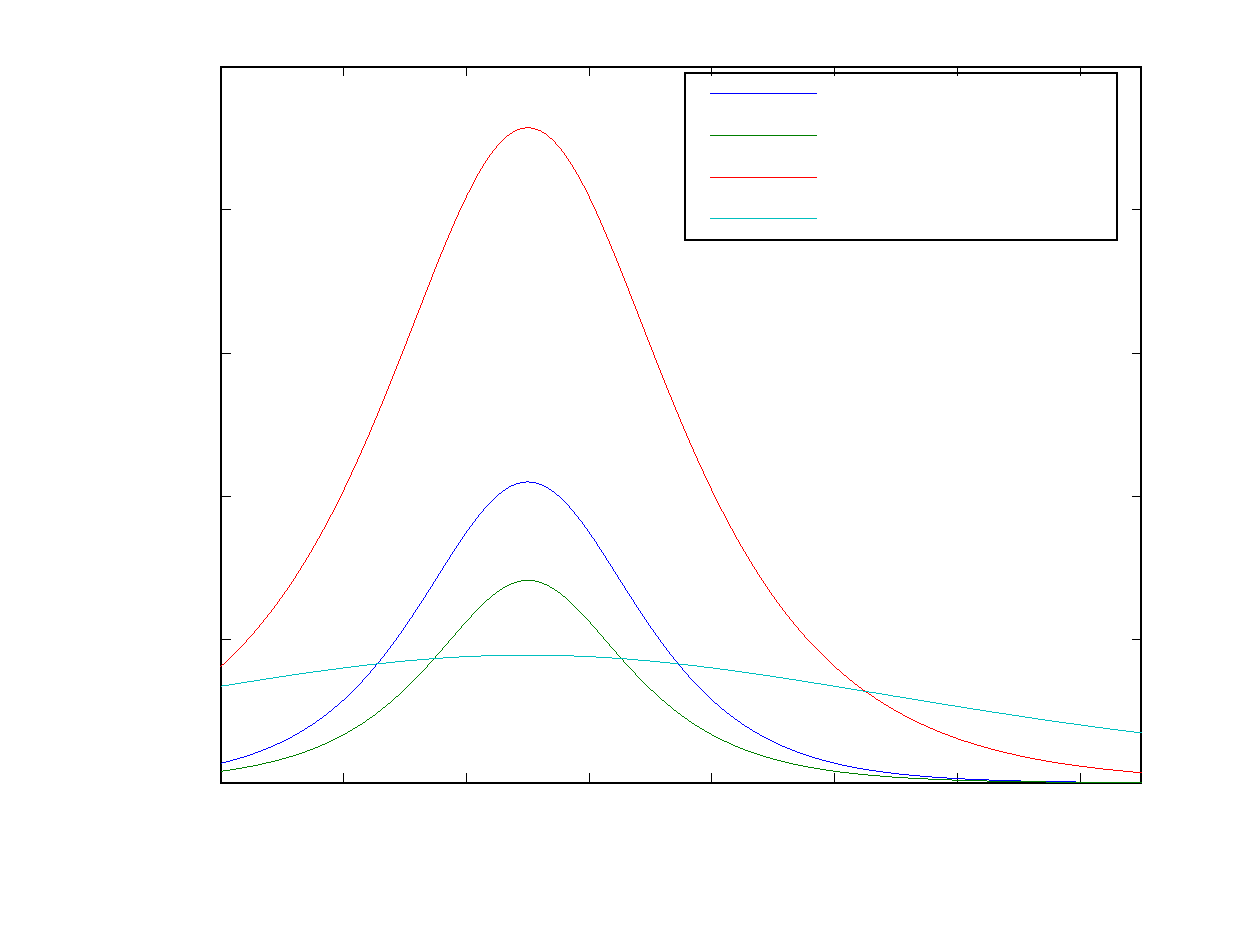
\includegraphics[width=0.6\textwidth]{chapter6/Images/MoveFlatnesses.eps}
				\caption{Manipulating the Spectral Flatnesses of the Test Signals.}
				\label{fig:MoveFlatnesses}
			\end{figure}

			The maximum flatness which can be achieved depends on the flatnesses of the two sets $L$ and $H$.
			If these sets are themselves flat (i.e. all partials in them have similar amplitudes) the maximum
			possible flatness will be large. If amplitudes of partials within each set have high variance the
			capacity for increasing the overall flatness is reduced.

			Equation \ref{eq:FlatnessManipulation} provides control over the spectral flatness in a signal
			where the amplitudes of the spectral components are known. As with control of spectral irregularity
			an analysis / synthesis technique could be utilised to implement this using harmonic excitation.
			Again it is desirable to remove the analysis step in order to reduce the complexity of the system.
			This can be done by replacing a band of spectral components with excited ones.

			Once a band has been replaced with excited components, the levels of these components can then be
			manipulated to change the flatness of the entire signal. Altering the flatness of the excited band
			using the method in Section \ref{sec:FeatureControl-Parameterisation-Flatness} changes the
			arithmetic mean of the components' amplitudes in the excited band while keeping their geometric
			mean the same. This causes the arithmetic mean of the amplitudes in the entire signal to change in
			the same direction while the geometric mean is unchanged. In short, increasing the flatness of the
			excited band will also increase the flatness of the entire signal and decreasing the flatness of
			the band decreases the flatness of the signal.

			As the spectral flatness measure doesn't depend on the frequencies of the spectral components
			deciding what two groups of components to apply reciprocal gains to will depend on the desired
			effect on other spectral features. For instance, to have a maximal effect on the odd to even
			harmonic ratio one could select two groups which consist of odd and even harmonics respectively. To
			have a minimal effect on this feature the two groups can both consist of one parity of harmonic.

	\subsection{Spectral Slope}
	\label{sec:FeatureControl-Parameterisation-Slope}
		The spectral slope measures the gradient of the spectrum. It is calculated by first order liner regression
		of the spectrum. For a signal with $N$ spectral components the spectral slope can be calculated with
		Equation \ref{eq:SpectralSlope}.

		\[ A = \sum_{n = 1}^{N} 20\log (a_{n}) \quad B = \sum_{n = 1}^{N} 20\nu_{n}\log (a_{n}) \]
		\[ F = \sum_{n = 1}^{N} \nu_{n} \quad G = \sum_{n = 1}^{N} \nu_{n}^{2} \]
		\begin{equation}
			S = \frac{NB - FA}
		                 {NG - F^{2}}
			\label{eq:SpectralSlope}
		\end{equation}

		Where $a_{n}$ and $\nu_{n}$ are the amplitude and frequency of the $n$\super{th} spectral component.

		Negative values of spectral slope describe a spectrum where the majority of the energy is in the low end of
		the spectrum. Positive values describe signals with more energy in the high end of the spectrum. A value of
		zero describes either a signal where the energy is evenly distributed throughout the spectrum or one in
		which the majority of the energy is in the middle of the spectrum.

		Traditional measures of spectral slope take a linear regression of the DFT bins. For musical signals which
		are composed of partials it may be more beneficial to measure the slope of the partial's amplitudes rather
		than of the whole spectrum. It is also common to measure how the amplitudes of partials decrease with
		frequency in dB per octave. Equation \ref{eq:SpectralSlope} can be altered to produce values in this unit
		by using the $\log_{2}$ of the frequency.
		
		\subsubsection*{Manipulation of Spectral Slope}
			As discussed in Section \ref{sec:ExcitationEvaluation-Comparison-SpectralCharacteristics} the
			spectral slope of the band of distortion components generated using a static nonlinearity depends
			on the continuity of the nonlinearity's characteristic curve and its derivatives. Using a simple
			system, similar to that in Figure \ref{fig:F0Tracking}, the characteristic curve of the
			nonlinearity can be changed to influence the spectral slope of the output signal.

			The system shown in Figure \ref{fig:InharmonicitySystem} provides more control, allowing for slopes
			other than multiples of 6dB per octave. As with the discussions on spectral irregularity and
			flatness the best way to control spectral slope in a signal is through analysis and resynthesis.
			To increase the spectral slope by $k$, each spectral component in the signal should have its
			amplitude, $a_{n}$, multiplied by the value $10^{\frac{1}{20}(k\nu_{n} - k\nu_{1})}$. Figure
			\ref{fig:MoveSlopes} shows the manipulation of the spectral slopes of the test signals.

			\begin{figure}[h!]
				\centering
				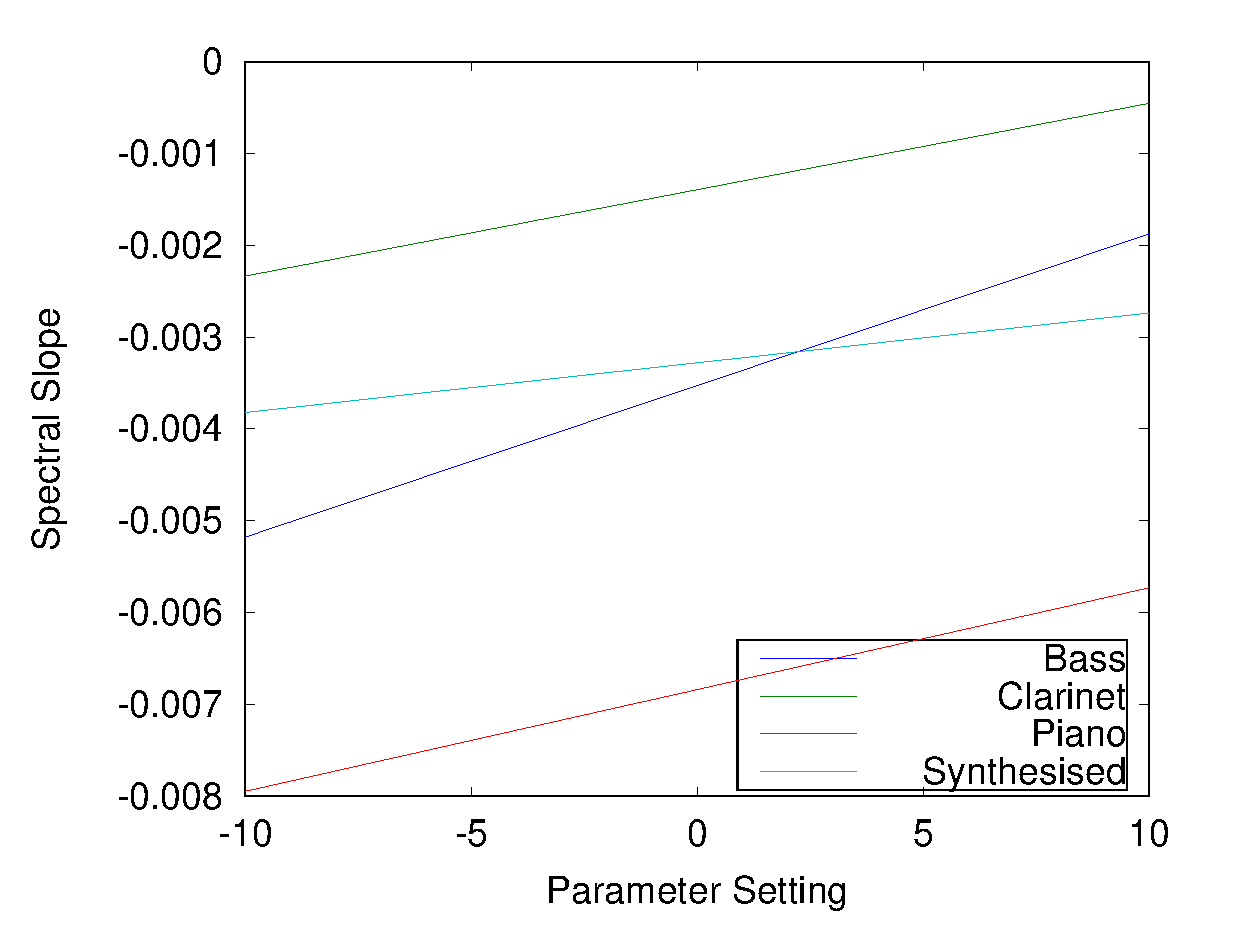
\includegraphics[width=0.6\textwidth]{chapter6/Images/MoveSlopes.eps}
				\caption{Manipulating the Spectral Slopes of the Test Signals.}
				\label{fig:MoveSlopes}
			\end{figure}

			Ideally each line in Figure \ref{fig:MoveSlopes} would have the same gradient as the signals'
			spectral slopes are being increased by the same factor. They do not however as only the fist nine
			harmonics are being individually manipulated. The differences in amplitudes of the higher order
			harmonics between the signals account for the differences in control of the spectral slope.

			If measuring spectral slope in dB per octave, to increase the slope by $k$dB per octave, each
			spectral component in the signal should have its amplitude, $a_{n}$, multiplied by the value
			$10^{\frac{1}{20}(k\log_{2}(\nu_{n}) - k\log_{2}(\nu_{1}))}$.

			If the analysis section is removed the excited spectral components can have their amplitudes set to
			give the desired slope. This is achievable for the lower order harmonics which are generated
			individually.  The static nonlinearity used to generate the higher order harmonics should be chosen
			to produce a band with a roll off as close to that of the desired slope. Generating the high order
			harmonics in this manner reduces complexity at the cost of accurate control of the spectral slope.

%\section{Controlling Features with Exciters}
%\label{sec:FeatureControl-Control}
%	This section will take the systems discussed in Section \ref{sec:FeatureControl-Systems} and use them to alter
%	audio features using the parametrisation techniques given in Section \ref{sec:FeatureControl-Parameterisation}.
%	The system shown in Figure \ref{fig:InharmonicitySystem} provides sufficient flexibility for implementing the
%	majority of these manipulations. The full extent of this system is not needed for some of the simpler modifications
%	so various subsystems of it are used.
